\documentclass[12pt]{article}
\linespread{1.5}
\pdfminorversion=6

\usepackage{booktabs}
\usepackage{tabularx}
\usepackage{caption}
\usepackage[flushleft]{threeparttable}
\usepackage{threeparttablex}

\usepackage[english]{babel}
\usepackage{float,color}
\usepackage[pdftex]{graphicx}
\usepackage{hyperref}
\usepackage{graphicx,scalerel}
\hypersetup{colorlinks,linkcolor=black,urlcolor=blue,citecolor=black}
\usepackage{amssymb}
\usepackage{amsmath}
\usepackage{placeins}
\usepackage[format=hang,font=normalsize,labelfont=bf]{caption}
\usepackage[margin=1in]{geometry}
\usepackage{url}
\usepackage{listings}
\usepackage{amsxtra}
\usepackage{setspace}
\usepackage{authblk}
\usepackage{csquotes}

% Bibliography stuff
\usepackage[
hyperref=true,
giveninits=true, % render first and middle names as initials
uniquename=init,
maxcitenames=3,
maxbibnames=99,
style=authoryear,
dashed=false, % re-print recurring author names in bibliography
natbib=true,
useprefix=true, % for inclusion of 'de' 'da' in surname
urldate=long,
backend=biber,
style=apa]{biblatex}
\addbibresource{bibliography.bib}


% adds space above row
\newcommand{\customlinespace}{\addlinespace[.1cm]}

% command for all table/figure notes
\newcommand{\Fignote}[1]{
	\begin{tablenotes}[para,flushleft]\footnotesize
		\textit{Note}: #1
	\end{tablenotes}
}

% stars
\newcommand{\sym}[1]{\rlap{#1}}

% note addendem for regression tables
\newcommand{\Regnote}{Standard errors in parentheses are clustered at the zip code level. ***, **, and * indicate significance at the 1, 5, and 10 percent critical levels, respectively.}


% Title page stuff
\title{The Effect of the Cook County, Illinois Tax on Sugar-Sweetened Beverages on Sugar Consumption}
\author{Zachary A. Goodman\thanks{zgoodman@ucsd.edu}\\ and Jacob Orchard\thanks{jdorchard@ucsd.edu. We gratefully recognize Prashant Bharadwaj, Jeffrey Clemens, Gordon Dahl, Itzik Fadlon, Mark Jacobsen, Katherine Meckel, Kaspar Wuthrich, and numerous seminar participants for their helpful comments and suggestions. Our analyses are calculated based in part on data from Nielsen Consumer LLC and marketing databases provided through the NielsenIQ Datasets at the Kilts Center for Marketing Data Center at The University of Chicago Booth School of Business. The conclusions drawn from the NielsenIQ data are those of our own and do not reflect the views of NielsenIQ. NielsenIQ is not responsible for, had no role in, and was not involved in analyzing and preparing the results reported herein.}}
\affil{University of California, San Diego}
\date{This version: April 2021}

\begin{document}
\maketitle

\begin{abstract}
Between 2015 and 2018, Sugar Sweetened Beverage (SSB) taxes were enacted in eight localities in the United States varying from one to two cents per ounce. In this paper, we examine whether SSB taxes achieve the goal purported by supporters: reducing sugar consumption. We use household scanner data to estimate the effect of SSB taxes on sugar purchases. We find that each additional cent per ounce tax decreases sugar purchases across grocery store products by TODO\%, TODO\% of which is explained by reduced purchases of sugar from beverages. We document stockpiling behavior and cross-border shopping as two mechanisms consumers employ to reduce their tax burdens.
\end{abstract}

\pagebreak

\doublespacing

%%%%%%%%%%%%%%%%%%%%%%%%%%%%%%%
% Introduction
%%%%%%%%%%%%%%%%%%%%%%%%%%%%%%%
\section{Introduction} \label{introduction}

Obesity remains among the costliest health issues in the United States today. \textcite{finkelstein2009annual} find that obesity related health expenses cost the U.S. between \$101 billion to \$173 billion in 2008 in 2018 dollars. \textcite{cawley2012medical} estimate significantly larger aggregate expenses totaling \$246 billion using an IV approach.  As a potential solution to reducing the high medical costs of obesity, government agencies have relatively recently suggested reducing added sugar consumption \parencite{dietary2015dietary}. Sugar sweetened beverages (SSBs) are the source of nearly 40\% of the average American's consumption of added sugar \parencite{dietary2015dietary} and about 7\% of caloric intake \parencite{allcott2019should}, several policymakers have recommended imposing taxes on SSBs to drive down sugar consumption and health costs.

While excise taxes on soft drink taxes have existed for many years in the U.S. and other countries, SSB taxes of the magnitudes examined in this paper (one to two-cents-per-ounce) began as recently as 2015 in the U.S. in Berkeley, California. Since then, several localities have followed in passing SSB taxes including Albany, California; Boulder, Colorado; Cook County, Illinois (home of Chicago); Oakland, California; Philadelphia, Pennsylvania; San Francisco, California; and Seattle, Washington. Despite these policy changes, the impacts of SSB taxes on the policy-relevant metric of sugar consumption have not yet been widely examined in peer-reviewed literature.

In this paper, our primary outcome of interest is the effect of SSB taxes enacted in the U.S. between 2015 and 2018 on total grams of sugar purchased. We use a large representative panel dataset with detailed purchase data and exploit variation across time and space in a differences-in-differences specification to complete our analysis. We find that on average, a one-cent per ounce increase in an SSB tax reduces total sugar purchases by TODO\%. Additionally, we find evidence that TODO.

Although most of the SSB taxes passed in the U.S. were passed by voter referenda rather than by local government officials, the policies have been highly controversial. Proponents of these measures have argued that like taxes on tobacco products, taxes on SSBs could be effective in improving public health while raising revenues that could be used for health education. Opponents have argued that the tax is poorly targeted given that consumers can substitute towards other sugary goods instead of beverages or simply evade the tax by shopping outside the borders of the taxed locality. Additionally, opponents have contended that the taxes would be regressive since SSBs constitute a larger share of poorer consumers' budgets than they do for those with more resources. In this paper, we do not take a stance on welfare changes, but we do find TODO.

The remainder of the paper is organized as follows. Section \ref{background} provides a background of the policies enacted and related literature. Sections \ref{methods} and \ref{data} introduce the methods and data used, respectively. Section \ref{results} summarizes our results. Section \ref{discussion} discusses those results, and Section \ref{conclusion} concludes.

%%%%%%%%%%%%%%%%%%%%%%%%%%%%%%%
% Background
%%%%%%%%%%%%%%%%%%%%%%%%%%%%%%%
\section{Background and Related Literature} \label{background}

In this section, we provide background on beverage taxes in the United States and summarize existing related literature.

\subsection{Beverage Taxes in the United States}

While dozens of cities have considered taxing beverages, the first city to pass an SSB tax was Berkeley, California in November 2014. Berkeley's Measure D levied a one-cent-per-ounce excise tax on the distribution of beverages with added sugar. Alcohol, milk products, beverages for medical use, 100\% fruit and vegetable juices, water, and artificially sweetened beverages are all exempt from the tax. The tax had been announced to begin January 1, 2015, but implementation was delayed until March of 2015 \parencite{falbe2015higher}.

Nearly two years after Berkeley, other cities began enacting similar SSB taxes including Philadelphia, PA, (2017); Oakland, CA, (2017); Albany, CA (2017); Boulder, CO, (2017); San Francisco, CA, (2018); Seattle, WA, (2018). Cook County, IL, which includes Chicago, became the first county to enact a county-wide SSB tax on August 2 of 2017. Two months later on December 1, the county became the first locality in the United States to end an SSB tax. One can observe a timeline of SSB tax events in Figure \ref{taxtimeline} below.

\begin{figure}[t]\centering
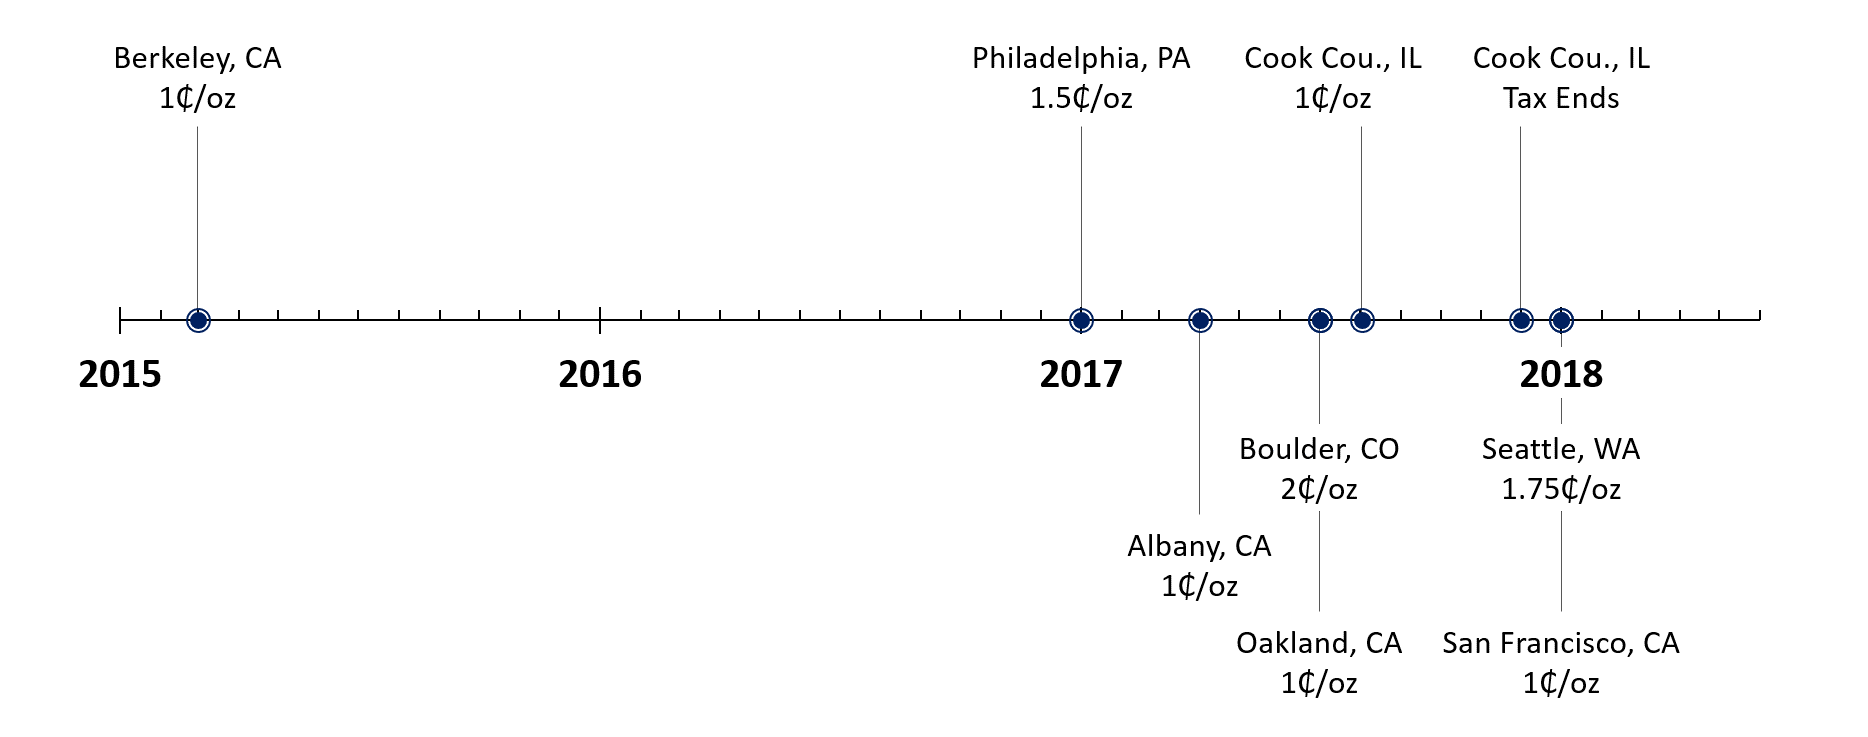
\includegraphics[width = \textwidth]{../figures/taxtimeline.png}
\caption{Rollout of SSB taxes in the United States \label{taxtimeline}}
\end{figure}

\subsubsection{Berkeley, California}

Each of the aforementioned studies find evidence that the tax in Berkeley resulted in high passthrough of the tax to consumers, which reduced SSB consumption. From these findings we learn that consumers are not perfectly elastic in their demand for SSBs, but we cannot say whether the taxes reduced sugar consumption because the authors did not examine demand interrelationships with other goods that contain sugar. About 39\% of the average American's daily sugar consumption comes from beverages that are taxable under the examined policies \parencite{dietary2015dietary}. It would be a problem for policymakers if, for example, taxed consumers substituted away from soda towards chocolate milk or candy. These studies also suffer from only sampling consumers in one region and failing to track where consumers purchase SSBs, which may have changed following the tax.

\subsubsection{Cook County, Illinois}

As the lone county-enacted tax, lone repealed tax, and largest tax by geography and number of constituients affected, we provide some additional background on the Cook County SSB tax.

The Cook County Board of Commissioners passed the Cook County Sweetened Beverage Tax Ordinance with a 9-8 vote on November 10, 2016. Initially, the one-cent-per-ounce tax was slated to go into effect on July 1, 2017; however, just four days earlier on June 27, the Illinois Retail Merchants Association filed suit, questioning the constitutionality of the tax. A state judge issued a temporary restraining order on the new tax until the case could be reviewed. On July 28, the same judge dismissed the lawsuit, and shortly thereafter on August 2, 2017, the beverage tax went into effect. As Cook County is home to 5.2 million residents, this tax became the most widespread SSB tax in the United States.

The Cook County beverage tax is unique among the other beverage taxes in the U.S. Besides having impacted the largest U.S. population to date, the law required that the tax be ``borne by the purchaser of the sweetened beverage," (Cook Co. Board of Commissioners, 2016). In practice, this meant that although the tax was collected by distributors, the law required that the tax be added to the price faced by consumers, usually in the form of a line-item on the receipt. This element of the policy has important implications for pass through and salience. Several large chain retailers added to the price tags of beverages a disclaimer that the tax would be added at the register (see Appendix \ref{pricetag} for an example.) However, it is possible that many retailers added the tax at checkout without including the tax in the displayed price, which may have reduced salience of the tax and possibly the impact on consumption \parencite{chetty2009salience}.

Importantly, the Cook County beverage tax was not levied on products purchased using SNAP benefits since federal law prohibits taxation of these goods. All other localities in the US that have enacted SSB taxes levied them on distributors - NOT consumers directly - and did not require that the tax be added at the register. As we will discuss in the next subsection, authors have found evidence of less than 100\% pass through in these localities. Additionally, because these taxes are levied on distributors, the passed-through portion of the taxes could be paid for using SNAP benefits. Hence, the level at which the beverage tax is levied is a policy lever that can be used to possibly address regressivity concerns or subsidize a local-government budget with money from federal transfer programs. Another element to consider is that poorer folk most likely to receive SNAP benefits are also those most likely to face the nutrition informational barriers that drive internalities from SSB consumption (Allcott, Lockwood, \& Taubinsky, 2019b). If so, then exempting SNAP benefits from the tax may actually hurt consumers.

To grasp the magnitude of the tax in Cook County, consider some popular beverages from our data. The most popular (in gross sales) carbonated beverage in our data for Cook County consumers is a 12-pack of 12-ounce cans that retails for \$3.57 on average. The Cook County beverage tax adds \$1.44, or 40\%, to the price of this 12-pack on average. The next most popular carbonated beverage is self-serve fountain beverages of assorted sizes, which retail for \$1.69 on average. For 20 - 32 ounce fountain drinks, the tax would add approximately 12\% - 19\% to the price. The most popular two-liter carbonated beverage retails for \$1.42 on average, and the tax adds 48\% to the price of this 67.6-ounce product. Considering taxed non-carbonated soft drinks, the most popular beverage is a 59-ounce lemonade product that retails for \$2.35 before the tax, or 25\% more with the tax. Across all carbonated beverages purchased in our dataset, we estimate the average percent tax to be about 23.5\%.\footnote{We only include carbonated beverages in this calculation since our data code both taxed and untaxed non-carbonated soft drinks together. Fruit-flavored juices ($<$100\% juice) tend to be cheaper per ounce than carbonated beverages, hence the percent tax is likely higher than the estimate reported here.}

Is is worth noting that Chicago, circumscribed within Cook County, has levied a 3\% tax on non-fountain soft drinks (paid by consumer) as well as a 9\% tax on wholesale fountain drink syrups (paid by distributor) since 1994. These taxes are in addition to an Illinois state sales tax of 6.25\%, Cook County sales tax of 1.75\%, Chicago sales tax of 1.25\%, and a Regional Transit Authority (RTA) tax of 1\%. The Cook County beverage tax studied in this paper is in addition to these aforementioned taxes. Note that the other taxes do not change during the period studied (2017).

Another difference between the Cook County tax and beverage taxes in other localities is the taxation of both regular and diet beverages. Besides Philadelphia, Pennsylvania, Cook County is the only other locality in the US to have included diet beverages in its beverage tax. Since diet beverages are close substitutes for regular beverages but contain no sugar, taxing them may be counterproductive if the goal is reduced sugar consumption. On the other hand, if maximizing revenue is the primary goal, then taxing diet beverages is likely a dominant policy strategy.

On October 11, 2017, the Cook County Board of Commissioners voted 15-2 to repeal the ordinance, becoming the first governing body in history to revoke a beverage tax. The one-cent-per-ounce tax expired on December 1, 2017.

\subsubsection{Other localities} \label{otherlocalities}

The Berkeley tax is the longest standing SSB tax in the U.S., and the most studied for its impact on consumption. \textcite{falbe2015higher} randomly surveyed retail establishments in San Francisco, Oakland, and Berkeley both before and after the tax change and found that the one-cent-per-ounce tax led to 0.46-0.67 cent increase in the price per ounce, depending on the type of beverage. In a follow-up study, \textcite{falbe2016impact} used a repeated cross-sectional survey of low-income and minority households before and after the tax. Participants were asked how often they consume different types of beverages each week or month, and total SSB consumption was inferred from their responses. The authors found that SSB consumption decreased by 21\% in Berkeley while it increased by 4\% in comparison cities. \textcite{silver2017changes} used store surveys and point-of-sale scanner data for three Berkeley and six non-Berkeley supermarkets to assess the tax pass through. They found that the tax pass-through was near 100\% for large chain supermarkets and smaller for others. They also found that sales of SSBs decreased in Berkeley relative to other cities. \textcite{cawley2017berkeley} add to the literature that stores in Berkeley pass through more of the tax to consumers the further away they are from borders with neighboring untaxed localities, ceteris paribus.

Each of the aforementioned studies find evidence that the tax in Berkeley resulted in high, but not 100\%, pass-through of the tax to consumers, which reduced SSB consumption. From these findings we learn that consumers are not perfectly elastic in their demand for SSBs, but we cannot say whether the taxes reduced sugar consumption because the authors did not examine demand interrelationships with other goods that contain sugar. While about 39\% of the average American's daily sugar consumption \parencite{dietary2015dietary} and about 7\% of daily calories \parencite{allcott2019should} come from beverages that are taxable under the examined policies, it would be a problem for policymakers if, for example, taxed consumers substituted away from soda towards chocolate milk or candy. Most of these studies also suffer from only sampling consumers in one region and failing to track where consumers purchase SSBs, which may have changed following the tax. Additionally, these studies rely on survey data, which likely contain significant response bias. Given the increased attention of the potential negative health effects of SSBs and respondents' tendencies to provide prosocial answers to surveyors\footnote{Researchers have observed that people tend to overreport socially positive behaviors like voting \parencite{silver1986overreports} and attending church \parencite{hadaway1993polls} but underreport socially negative behaviors like declaring bankruptcy \parencite{locander1976investigation} and using illegal drugs \parencite{mensch1988underreporting}. See \textcite{krumpal2013determinants} for a review of the literature on ``Social Desirability Bias."}, it would not be surprising to find that respondents underreport their SSB consumption to a larger degree following implementation of the tax.

More recently, other authors have examined the SSB taxes in Boulder \parencite{cawley2020boulder}, Oakland \parencite{cawley2020oakland}, and Philadelphia \parencite{cawley2020philly}. In Boulder, Cawley and coauthors find that nearly 80\% of the two-cents-per-ounce tax in Boulder was passed on to the consumer. Importantly, they note that about one-fifth of the retailers surveyed added the SSB tax at the register rather than into the shelf-price, which may have reduced saliency of the tax, perhaps lowering its effectiveness \parencite{chetty2009salience}. In Oakland, TODO. In Philadelphia, the authors find that consumers purchased 8.9 ounces of SSBs per shopping trip less from stores within the city relative to consumers who purchased SSBs from stores outside the city. They also find evidence that city residents increased their purchases of SSBs outside the city.

One important variation between the taxes examined in this paper is whether or not sugar-free diet beverages are taxed, which is the case in the Cook County and Philadelphia SSB taxes. As such, we investigate heterogeneity in substitution along this difference. Future work that examines the impact of SSB taxes on weight loss will need to consider this difference as well. Finally, it is important to note that all of the policies enacted exempt alcohol, baby formula, beverages in which milk is the first ingredient, beverages used for medical purposes, and 100\% fruit and vegetable juices. Several of these products contain nontrivial quantities of sugar or carry externalities that may outweigh the reductions in obesity-related social costs.

\subsection{Effect of SSB taxes on health}

An often reported goal of SSB tax supporters is to reduce consumption of sugar. While there may be other mechanisms through which decreasing consumption of SSBs improves health, such as encouraging substitution towards more nutrient-dense foods, reducing total caloric consumption, and reducing consumption of other potentially health-harming ingredients present in SSBs, we focus our attention on the mechanism of decreasing sugar consumption. In this section, we provide background on the evidence that decreasing sugar consumption improves health and the ways by which SSB taxes may or may not reduce sugar consumption.

\subsubsection{Effect of sugar consumption on health}

TODO direct link papers

Two randomized controlled trials have directly tested the effect of SSBs on obesity. \textcite{ebbeling2012randomized} provided half of 224 overweight adolescents with a multicomponent intervention to reduce SSB consumption including home delivery of water and non-nutritive sweetened beverages (NNSBs) and regular phone calls and check-in visits. Control participants were provided \$50 supermarket gift cards twice over the year-long period. By the end of the intervention, treated participants reduced their consumption from over 1.7 SSBs per day to nearly zero whereas control participant SSB consumption remained greater than zero. The authors find that treatment reduced endline BMI by two percentage points more than control participants' BMI loss. In another experiment, \textcite{de2012trial} provided 641 children with 8 ounce cans of sweetened beverages daily, half of which were SSBs and the other half NNSBs. Participants were not made aware of how their beverages were sweetened as the can labeling was made consistent across conditions. The authors estimate that participants assigned to the SSB condition gained 19 - 35\% more bodyfat than did those assigned to the NNSB condition.

In both experiments, the authors examine the effect of SSBs versus experimenter-provided NNSBs on weight loss. This nudged substitution is unlike supermarket conditions where consumers face nonzero prices for noncaloric beverages, so it is not obvious that consumers would respond to SSB taxes by substituting towards sugar-free products. However, it is reasonable that consumers may substitute towards other sweet products. It is generally accepted in the scientific community that sweetness carries a signal of nutrient density, which through evolution has endowed animals with an innate preference for sweet foods. Furthermore, scientists have produced evidence that sweetness can be addicting in animals (see \textcite{avena2008evidence} for a review). The addictive properties of sweetness are not unique to sugar. \textcite{lenoir2007intense} find that 94\% of the rats employed in their study preferred saccharin-sweetened water over intravenous cocaine when provided both options and after having experienced both substances for several days.

If the findings from these animal models apply to humans, then one should \textit{expect} humans to seek sweetness elsewhere if not in the form of SSBs. Indeed, medical researchers have identified evidence of ``reward homeostasis," which if imbalanced can cause seeking of food-derived pleasure even in the absence of hunger (see \textcite{bellisle2012sweetness} for a review). This theory predicts that food satiation is a function of both calories consumed and achieving an individual's expected level of sweet-tasting foods. In one test of this theory, \textcite{lemmens2009eating} found that fasted subjects who were provided chocolate mousse instead of an isocaloric cottage cheese of the same weight subjectively reported less hunger and less desire for additional food.

The implication of this theory is that policies that make sugary foods more expensive while maintaining or even lowering the price of non-sugary, sweet foods (i.e. artificially sweetened foods) would help consumers achieve ``reward homeostasis" and reduce calories sought whilst not hungry. Hence, SSB taxes may be more effective at reducing obesity if diet beverages, which provided sweetness but no calories, are available as lower cost substitute beverages. This idea has been tested experimentally by  \textcite{peters2014effects} and \textcite{peters2016effects} who provided overweight, diet-beverage consumers vouchers for either diet beverages (treatment group) or water (control group) and asked them to consume at least 24 ounces of their assigned beverage per day for one year concurrent with enrollment in a weight loss program. At the end of the one year trial, the treatment group had lost 6.6\% of initial bodyweight while the control group had lost 2.6\%. Although the authors did not collect food diary data and thus cannot examine whether participants assigned to the water condition consumed more sugary goods, the experiment provides suggestive evidence that diet beverages may help consumers maintain reward homeostasis without consuming sugar. On the other hand, taxing diet beverages increases collected revenues, which may be an important element of the policymaker's objective function.

\subsubsection{How SSB taxes reduce sugar consumption}

For SSB taxes to be effective reducing sugar consumption, several mechanisms must function simultaneously. First, the tax must decrease SSB consumption. If the tax pass-through rate is low, or if consumers are very inelastic in their demand for SSBs, then the tax may have little impact on SSB consumption. As mentioned in Section \ref{otherlocalities}, existing research has validated that indeed, the pass-through rate is high and consumers do reduce their purchases of SSBs when prices increase. In this paper, we emphasize another potential mechanism through which consumers may not significantly reduce their SSB consumption: shopping at untaxed grocery stores. It is conceivable that consumers who shop regularly outside their localities may be unaffected by SSB taxes, or even that consumers may begin shopping at different stores following the tax, as \textcite{cawley2020philly} found in Philadelphia. Our data are less likely to contain reporting bias given that subjects are incentivized to report all purchases whereas participants may under report their consumption of untaxed SSBs to a surveyor located in a taxed locality.

Even if the tax manages to reduce consumption of SSBs, consumers can offset the decrease in sugar consumed from beverages by consuming more sugar from other foods. Indeed, about 68\% of US packaged foods and beverages (by caloric share) contain caloric sweeteners \parencite{popkin2016sweetening}, which may make it challenging for households substituting away from SSBs to select products that do not contain sugar.

%%%%%%%%%%%%%%%%%%%%%%%%%%%%%%%
% Methods
%%%%%%%%%%%%%%%%%%%%%%%%%%%%%%%

\section{Methods} \label{methods}

\subsection{Pass-through}

As the Cook County beverage tax is yet to be reviewed in the economics literature, we first begin by estimating the pass-through of the tax. We estimate the pass-through using the following specification, following the methods of Harding, Leibtag, and Lovenheim (2012):

\begin{align}
	P_{uist} = \beta_0 + \beta_1\tau_{st} + \alpha_u + \gamma_s + \lambda_t + \theta \mathbf{X}_{it} + v_{uist} \label{passthrough}
\end{align}

where $P_{uist}$ is the price of a product with UPC $u$ paid by household $i$ in county $s$ and month $t$, $\tau_{st}$ is the beverage tax in a county-month with units cents-per-ounce, and $\mathbf{X}_{it}$ is a vector of household-level controls\footnote{Household-level controls include age, presence of children, education, female and male head employment, presence of female and male heads, household income, race, and household size. Summary statistics for each control variable are presented in the next section. We only include households who do not move across counties, so we drop the county subscript for the control variables since they are location invariant.}. Notably, Equation \ref{passthrough} includes fixed effects for month, county, and UPC, which permits identification of the change in price \textit{for the same product} across time and location. This especially matters if, for example, consumers move to higher quality beverages following implementation of a tax that is levied by volume rather than percent of sale price.

To examine regressivity, we add an interaction term between $\tau_{st}$ and dummies representing income bins, which are included in the vector of controls, $\mathbf{X}_{it}$. Doing so enables us to identify whether the burden of the tax was greater for poorer or wealthier consumers while controlling for changes to quality of the bundle of goods purchased.

\subsection{Effect on sugar}

Next, we use a differences-in-differences specification to examine the impact of the tax on sugar purchases. We compare the change in monthly sugar purchases following introduction of the beverage tax by households living in Cook County, Illinois to that among those living in other counties that do not have a beverage tax. We do include San Francisco and Seattle in the counterfactual as neither city has levied a beverage tax during the period we observe in the data. % As a robustness check, we additionally use as a counterfactual the remainder of a Metropolitan Statistical Area (MSA) that contains a treated locality. For example, panelists in Wilmington, Delaware live in the same MSA as those in Philadelphia, Pennsylvania and hence are included in the control group.
Our specification is as follows:
\begin{align}
	\sigma_{ist} = \Delta_0 + \Delta_1 \tau_{st} + \delta_s + \psi_t + \theta \mathbf{X}_{it} + \varepsilon_{ist} \label{baseline}
\end{align}

where $\sigma_{ist}$ is the total grams of sugar across all products purchased by household $i$ in county $s$ during month $t$, and $\tau_{st}$ and $\mathbf{X}_{it}$ are defined the same as in Equation \ref{passthrough}. $\gamma_s$ and $\lambda_t$ are locality and time fixed effects, respectively. Observe that $\tau$ is only equal to one for households living in Cook County during the four months that the tax is in effect. Hence $\hat{\Delta}_1$ is the estimator of interest. If we assume that 1) the timing of the Cook County tax is not collinear with anything else that may have affected sugar purchases, 2) that the Cook County tax did not affect sugar purchases in counterfactual households (no spillovers), and 3) that the difference in sugar purchases between Cook County and counterfactual counties would have remained constant in the absence of treatment:
\begin{equation}
\begin{split}
\mathop{{}\mathbb{E}}\big[\sigma_{it,\: \text{Cook}} - \sigma_{it,\: \text{Counterfactual}}  |\: t<t^*\big] = \\
& \mathop{{}\mathbb{E}}\big[\sigma_{it,\: \text{Cook}} - \bar{\sigma}_{it,\: \text{Counterfactual}}  |\: t\geq t^*,\; \tau = 0\big] \label{didassume}
\end{split}
\end{equation}
where $t^*$ is the month the tax is first in effect, then $\hat{\Delta}_1$ can be interpreted as the causal average treatment effect of the Cook County tax on grams of sugar purchased for residents of Cook County during the taxed period. Note that the right hand side of Equation \ref{didassume} is unobservable and thus assumption 3) is fundamentally untestable. However, we can examine trends between Cook County and the counterfactual counties before the tax is implemented. Parallel pretrends does not prove assumption 3), but it gives us some confidence.

%A few assumptions must hold for this specification to identify the causal effect of SSB taxes on sugar consumption. Using the potential outcomes framework, we must assume that over the same time period, the observed change in sugar purchased by the control group is equal to what the (unobserved) change in sugar consumption would have been for the treated group in the absence of treatment. Although this assumption is fundamentally untestable, we can examine whether trends before the tax are parallel, which would provide confidence that our chosen control group is a sound counterfactual. In section 5 we demonstrate parallel pre-trends. Additionally, we assume errors are mean zero, normally distributed, and allow for correlation within localities, that is, the level at which the tax was assigned. We adjust our standard errors of our coefficient estimates by clustering at the locality level.

We consider adjustments to the standard DD specification in \eqref{baseline} by adding interaction terms to Equation \ref{baseline} to examine heterogeneous treatment effects:
\begin{align}
\sigma_{ist} = \Gamma_0 + \Gamma_1 \tau_{st} + \Gamma_2 \text{I}_{it} + \Gamma_3 \tau_{st} \text{I}_{it} + \delta_s + \psi_t + \theta \mathbf{X}_{it} + \varepsilon_{ist} \label{het}
\end{align}
where $\text{I}_{it}$ is a household-specific, location-invariant covariate of interest not included in the vector of household control variables $\mathbf{X}_{it}$. Specifically, we add interaction terms with income and race, which will help identify if the tax may have had differential effects across these demographic variables. Recall that SSBs purchased with SNAP benefits were not subject to the tax, so it is possible that the tax may have had no effect on poorer consumers most likely to receive SNAP benefits. We also create dummy variables that indicate the location of a household within Cook County using five-digit zip code identifiers. By letting $\text{I}_{it}$ be the household's ``layer" within the county, we can examine whether the policy had a lesser effect in locations closer to the border. Each layer is depicted in Figure \ref{cookzip} in the next section.

Finally, we let $\text{I}_{it}$ equal the pretax level of soda purchases. Doing so can be thought of as a triple difference specification where consumers with zero pretax soda purchases serve as an additional counterfactual layer. These consumers should not be affected by the Cook County tax yet face the same county-specific shocks that soda consumers experience. Hence, our identifying variation comes from changes in sugar consumption across counties, across time, and across exposure to the tax.

\subsection{Effect on quality, intensive margin, and substitution}

Since the SSB taxes are excised on a per-ounce basis rather than a percentage of value, the percent price increases of cheaper goods under the tax would be more than the percent price increases of more expensive goods, which may drive consumers to substitute towards higher cost SSBs (Harding, Leibtag, Lovenheim 2012). However, the negative income effect induced by the tax may cause greater consumption of relatively inferior SSBs. To examine changes in SSB quality, we will construct a quality measure by ranking products by average price (per ounce) across retailers. Note that if tax pass-through is consistent across products, then this ranking would not change after the tax is enacted since the per ounce prices would simply increase by the amount of the pass-through. We will estimate a specification similar to Equation \ref{baseline} except that the outcome variable of interest is $z_{ist}$, the average quality score of the products purchased by household $i$ in county $s$ during month $t$.

Another consideration, following the literature referenced earlier that humans have an innate desire for sweetness, is that consumers may substitute towards SSBs with higher concentrations of sugar per-ounce.\footnote{Consumers may employ other behaviors, such as reducing the amount of ice in one's cup when purchasing soft drinks, that affect the intensive margin but are unobservable in our data.} This would be consistent with the observed behavior of smokers who smoke cigarettes more intensively (extract more nicotine per cigarette) when cigarette taxes are increased (Adda \& Cornaglia, 2006). This substitution, if it exists, could help explain how SSB consumption could fall after tax implementation yet sugar purchases remain unchanged. To examine this margin, we calculate average grams of sugar per ounce of purchased beverages per month and use this as our outcome variable in Equation \ref{baseline}.

Finally, it is theoretically ambiguous whether consumers are more likely to consume more sugar from nonbeverages while the tax is in effect. On one hand, if sweetened beverages and nonbeverages are net substitutes, then some of the reduction in sugar from reduced consumption of SSBs should be offset by increased consumption of sweetened nonbeverages. On the other hand, imposing a tax as large as the one studied here may send a credible signal to consumers that sugar is unhealthy, which may cause consumers to update their preferences. If so, then consumers may substitute away from all sugary products including sugary nonbeverages. In this case, total sugar consumption would decrease by more than the amount that sugar from SSBs decrease. To answer this empirical question, we examine the impact of the tax on both total sugar and SSB sugar and compare the two estimates.

\subsection{Welfare}

While the above methods help us understand whether the tax may reduce sugar consumption and improve health, they do not capture the costs that households pay in the form of reduced consumption. To estimate the welfare loss from reduced consumption, we follow the structural approach of Redding and Weinstein (2018) to create price indexes. Compared to using a standard price level that assumes Cobb-Douglas utility and demand equal to constant budget share, the Redding and Weinstein method has the advantage of allowing for shifts in demand, prices, quality, variety, and consumer heterogeneity. We calculate price levels for both before and after the tax in both Cook and counterfactual counties. Each price index is determined using the following equation:
\begin{align}
P = \left[ \sum_k \left( \frac{p_k}{\varphi_k}  \right)^{1-\sigma}  \right]^{\frac{1}{1-\sigma}} \label{priceindex}
\end{align}
where $P$ is the price index, $\sigma$ is the elasticity of substitution across product modules, $p_k$ is the quantity-weighted average price within a product module, and $\varphi_k$ is the relative demand of each product module. After determining the four price levels (Cook vs. counterfactual, pretax vs. posttax), we can calculate the average compensating variation (in dollars) with:
\begin{align}
CV = \bar{C}\left(\frac{P_{1,\text{Cook}}}{P_{0,\text{Cook}}} - \frac{P_{1,\text{counterfactual}}}{P_{0,\text{counterfactual}}}\right) \label{cv}
\end{align}
where $\bar{C}$ is the average consumption (in dollars) among Cook residents in the pretax period. The intuition is as follows: suppose the price level to increases by 10\% in Cook County during the taxed period. Over the same time period, the price level increased in counterfactual counties by 6\%. Hence, in the absence of treatment, (we assume) the price level in Cook County would have increased by only 4\%, so the effective price increase caused by the tax is 4\%. To ``compensate'' the consumer for the increased prices (and return her to her baseline level of consumption), we must provide her with 4\% of the money she spent in the pretax period.

Interestingly, we can use this compensating variation to determine the social cost required to reduce sugar on a per-gram basis. Our measure will help policymakers conduct cost-benefit analyses of SSB taxes. These analyses must take into account 1) grams of sugar reduced per unit tax, 2) health cost savings per gram of sugar reduction, 3) compensating variation (social cost), and 4) transfers net transfer costs. This paper provides estimates of 1) and 3). We leave it to other researchers to determine the health cost savings per gram of sugar consumed (2) and policymakers to determine 4).

%%%%%%%%%%%%%%%%%%%%%%%%%%%%%%%
% Data
%%%%%%%%%%%%%%%%%%%%%%%%%%%%%%%
\section{Data} \label{data}

We identify the effects of SSB taxes by linking several data sources. First, we observe household-level food purchase and demographic data from the Nielsen Homescan Survey, a nationally representative panel of 40-60,000 households from 2004 to 2016. These data have been used to asses the effects of other taxes. \textcite{harding2012heterogeneous} use the homescan data to asses the impact of cigarette taxes, especially for panelists living close to state borders. \textcite{cotti2016effects} look at how tobacco taxes affect smoking cessation product purchases. \textcite{dharmasena2012intended} assess the effects of a hypothetical tax on sugar. \textcite{colchero2016beverage} and \textcite{colchero2017mexico} use Nielsen panel data in Mexico to evaluate the impact of a one-peso per liter tax on SSBs.

Nielsen provides recruited households with a handheld barcode scanner and asks them to record every item they purchase. By scanning their purchased products, households earn points that can be redeemed in a rewards catalog much like credit card reward programs. The households can earn higher value rewards the longer they remain in the panel, so households are additionally incentivized to participate in the panel for multiple years (the median household participation duration is about 7 years). Nielsen collects household characteristics including zip code level geographic identifiers, household size, age of household members, race, income range, residence type, and more. In Table \ref{panelist_dems}, we present descriptive statistics of households in the homescan data by SSB tax treatment status.

\begin{table}[htbp]\centering
\begin{tabular}{l*{3}{c}}
\hline\hline
	&\multicolumn{1}{c}{Treated}&\multicolumn{1}{c}{Control}&\multicolumn{1}{c}{Combined} \\
\hline
Under \$45K	&				0.36&				0.29&				0.30 \\
						&			(0.48)&			(0.45)&			(0.46) \\
\$45K - \$100K&				0.43&				0.46&				0.45 \\
						&			(0.49)&			(0.50)&			(0.50) \\
Over \$100K	&				0.21&				0.25&				0.24 \\
						&			(0.41)&			(0.43)&			(0.43) \\
Has children&				0.20&				0.28&				0.26 \\
						&			(0.40)&			(0.45)&			(0.44) \\
Married		 &				0.50&				0.65&				0.62 \\
						&			(0.50)&			(0.48)&			(0.49) \\
White			 &				0.63&				0.80&				0.76 \\
						&			(0.48)&			(0.40)&			(0.43) \\
Black			 &				0.26&				0.08&				0.12 \\
						&			(0.44)&			(0.27)&			(0.33) \\
\hline
\(N\)			 &				1754&				5746&				7500 \\
\hline\hline
\end{tabular}
\caption{Summary statistics for Nielsen households. Standard deviations are presented in parenthesis. \label{panelist_dems}}
\end{table}

Participants are asked to scan the UPC codes of \textit{all} the products they buy following shopping trips and provide information on the location of the purchase. If the purchase was completed at a Nielsen partner retail outlet, the price of the purchased item is automatically recorded as the average price of that product during the week that the customer recorded the purchase. If the purchase was made at a non-participating retail outlet, the participant is asked to manually input the price. If the product does not have a barcode as is the case with raw fruits and vegetables, households can record their purchase by scanning a barcode for the corresponding item printed in a provided booklet. Given that households may forget or choose to omit recording some of their purchases, the Nielsen Homescan Survey data likely contain measurement error. However, provided the measurement error is uncorrelated with introduction of SSB taxes, our findings, presented as percent changes, should remain unbiased. Levels of consumption presented in the data should be considered underestimates given the high likelihood of under-reporting by households \parencite{einav2010recording}.

We match the UPC codes from purchases in the Nielsen data with product-level nutrition data, thereby permitting us to observe total quantities of nutrients purchased by each household per month. Our nutrition data come from three sources. First, we use proprietary nutrition data from Syndigo, who provide UPC-level product information including the Nutrition Facts (amount of each micro and macronutrient listed), ingredients, product size, description, and brand for over 220,000 branded packages.\footnote{The data are licensed by over 2,000 consumer applications and have been used to estimate nutrients purchased by Nielsen panelists by other authors including TODO.} Second, we use the US Department of Agriculture's FoodData Central to gather nutrition information for foods that do not have Nutrition Facts (such as produce). Third, for remaining products, we use the search features of major online retailers to find images of the Nutrition Facts panel and manually record the information.

To match nutrition data to the Nielsen product data, we follow a procedure similar to that of \textcite{dubois2014prices}. We first drop non-food products, alcohol, tobacco, weight-loss/diet aids, and reference card goods.\footnote{Reference card goods are products without a barcode that panelists can report they purchased by scanning barcodes listed in a barcode reference booklet. These reference barcodes are associated with pictures and standardized item descriptions (such as ``bakery item"). We drop these products since we cannot infer accurate nutrition information, and reference card goods are vastly underreported relative to products that have barcodes. Nielsen provides alternative panelist weights for analyses that include reference card goods.} % As a robustness check we examine whether RC purchases change as a function of the tax.
We then match on UPC code, which matches about TODO of the purchased UPCs. Next, for products without a direct match, we match within brand, product module,\footnote{over 1,075 product categories defined by Nielsen}, size type (e.g. measured in counts versus milliliters versus grams), flavor, and formula. This step adds TODO to the matched data. Next, we allow the brand requirement to be flexible, which permits matching across store-brands and adds another TODO\%. The remaining TODO\% of unmatched goods are mostly random-weight items such as raw produce and single-serve baked goods.

%%%%%%%%%%%%%%%%%%%%%%%
% Results
%%%%%%%%%%%%%%%%%%%%%%%

\section{Results} \label{results}
In this section we present results using the methodology discussed in section 3 and data introduced in section 4.

\subsection{Pass-through}

First, we examine pass-through of the tax by estimating Equation \ref{passthrough}. Because the Nielsen data do not include tax in the recorded prices, we manually add the tax to the prices using the store zip code and week of purchase. However, store zip code is not observable in roughly half of the observations, so we first estimate Equation \ref{passthrough} with only the data from observations where the zip code is visible. Second, we code the zip codes of stores without zip codes to be the modal zip code among patrons during the pre-tax period.

Because the tax may have changed which beverages are purchased, and because we cannot observe which beverages are endogenously not purchased during the taxed period because of higher prices, we only include beverages that are purchased in both the pre-tax and post-tax period when estimating equation 1. Doing so avoids selection bias, but the result is representative only of the beverages contained in our sample. Theoretically, we should underestimate the passthrough as consumers substitute towards relatively cheaper beverages with lower rates of passthrough. A better strategy would be to examine retailer-level price data that contains prices of goods that go unpurchased in the consumer-level data.

Finally, we only include carbonated beverages as the vast majority of these beverages are taxable whereas other beverage categories (such as fruit juices) contain both taxed and untaxed products. In both specifications, we fail to reject a 100\% passthrough. We plot the time series in Figure \ref{pricechange} below.

\subsection{Effect on sugar}

Next, we estimate the effect of the tax on sugar purchases (from all food sources) using Equation \ref{baseline}. To instill some confidence that our comparison group is a credible counterfactual, we plot the time series of average monthly sugar purchases per household in Figure \ref{didsugar} below. One can see that nonparametrically, the difference between treatment and control on any given month pre-tax is statistically indistinguishable from zero. However, during the tax, the difference becomes statistically significantly different from zero. Interestingly, total sugar purchases appear to increase both immediately before and immediately after the tax is in effect; however, neither jump is significantly distinguishable from zero.

To examine whether this reduction came from reduced SSB consumption, we similarly plot the time series of total sugar purchased only from carbonated beverages (Figure \ref{didsugarsoda}). Much like the plot of total sugar, the plot of soda sugar includes steep decline during the taxed period surrounded by sharp spikes in the months before and after the taxed period. Directionally, it seems plausible that consumers did not entirely compensate for their reduced soda purchases with sugar consumption from elsewhere.

Our estimates for Equation \ref{baseline} using both total sugar and sugar from soda as outcome variables can be seen in Table \ref{didsugartable} below. We find that during the taxed period, consumers purchased 7.3\% less sugar overall when compared to purchases by consumers living in untaxed counties. Interestingly, we find that 58\% of the reduction in total sugar is explained by the reduction of sugar from regular carbonated beverages.\footnote{We are working on estimating total sugar from \textit{all} taxed beverages, which would help us determine if the remainder of this gap can be explained by reduction in taxed beverages alone or possibly changing consumer attitudes towards sugar consumption from sources other than beverages.} % TODO: use sugar from all beverages.

Next we will discuss two methods that consumers may have employed to avoid the tax: stocking-up before the tax, and traveling across the border to purchase beverages at untaxed stores.

It's plausible that rational, forward-looking agents anticipating the tax may have purchased large quantities of soon-to-be-taxed beverages before the tax went into effect, thereby avoiding the tax for at least a short while. These consumers could then smooth their consumption of taxed beverages throughout the beginning of the taxed period without paying any additional taxes. Since our data comprise \textit{purchases} and not \textit{consumption}, we cannot observe whether households consume pretax-levels of taxed beverages during the tax. However, we can observe the heaping of soda purchases in the months leading up to the tax and in the month after the tax is removed. Ignoring this stockpiling behavior would lead to overstatements of the effect of the tax on sugar consumption.

One method to estimating the effect of the tax is to use the announcement of the tax as the first ``treated" period instead of when the tax actually went into effect. However, the tax was passed in November of 2010, about nine months before the tax went into effect, which is longer than the shelf life of most of the taxed beverages. However, the Cook County tax is unique in that the effective date of the tax was delayed one month after a lawsuit was filed against the ordinance. Consumers found out that the tax would be delayed only \textit{four days} before it was slated to go into effect. Consumers attempting to maximize shelf-life subject to not paying the tax may have waited until the weeks before the tax is in effect to stockpile soda, which may have began in late June - over a month before the actual implementation date, but only a few days before the scheduled implementation date. This story is consistent with what we observe in the data: an increase in regular soda purchases in June that persists through July and drops off during the taxed period in August onwards.

We assume that agents seeking to avoid paying the tax would wait until the last month to stockpile. Besides increasing longevity of the supply during the taxed period, doing so carries less storage costs and additional option value of waiting (in case the tax is delayed or repealed, for example). Hence, we treat June as the first month that the forthcoming policy affects behavior, and we treat September as the last month since in October, the law is repealed, which may again change purchasing behavior. When we again estimate equation \ref{baseline} using this two-month earlier shifted period, we find that the tax reduced total sugar by 3.4\% and sugar from soda by 1.7\%. Point estimates and standard errors are presented in Table \ref{tableshortrun} below. We consider this estimate a more accurate estimate of the short run impact of the tax on sugar \textit{consumption}.

Next, we examine the importance of distance from untaxed stores with respect to the effectiveness of the tax at reducing sugar consumption. Theoretically, households near the border face lower costs to avoid the tax than do households in the center of the taxed county since the cost to travel to an untaxed store is lower. We estimate Equation \ref{het} after coding each household with an indicator variable for their zip-code border as depicted in Figure \ref{cookzip}. We present the coefficient estimates on the interaction term between the tax and the zip border dummy in Figures \ref{ziptotsugar} and \ref{zipsugarsoda} below, which estimate the effect of the tax on total sugar purchases and sugar from soda purchases, respectively. While the coefficient is indistinguishable from zero for households who live in a border or cross-border zip, the coefficients are negative and economically significant for three of the four protected zip code layers.

% Finally, we examine heterogeneity in treatment effects by household demographics.

%\subsection{Effect on quality, intensive margin, and substitution}

%%%%%%%%%%%%%%%%%%%%%%%
% Discussion
%%%%%%%%%%%%%%%%%%%%%%%
\section{Discussion} \label{discussion}

%We find that TODO.

% Robustness Checks
% NY State budget 18% in 2009 and 1c/oz in 2010 not passed. In NYC in Sept 2012, >16 oz beverages banned starting March 2013, but overturned by courts in March 2013 before implementation. Could examine trends in purchases...

\subsection{Limitations}

Our approach has a few limitations. We observe sugar purchases, not sugar consumption, which is the policy-relevant metric. However, if we assume that the fraction of sugar purchased to sugar consumed does not change following the tax, our estimate of the effect of the tax on sugar purchases would additionally estimate the effect on sugar consumption. This assumption could be violated if, for example, consumers buy less sugar after the tax is enacted but consume the same amount by consuming a greater portion of their purchased sugar. It is not possible to test this assumption using the Nielsen data, though violations of this assumption likely bias our estimates \textit{upwards} since consumers presumably start consuming a larger portion of the purchased sugar as it becomes relatively more expensive. Additionally, we cannot observe some intensive margin changes to soda consumption like consuming more soda from a container before disposal.

Additionally, we observe grocery store purchases that households scan, which does not include unscanned items such as food consumed away from home. Since SSB taxes studied in this paper are levied based on volume, SSBs sold at grocery stores are generally taxed at higher rates than are SSBs consumed at restaurants, which could result in substitution of SSB purchases away from home (TODO: cite existing literature on effect of taxes at restaurants). Finally, we do not examine health directly. While sugar consumption decreases during the taxed period, agents may simultaneously change other behaviors, such as exercise. Consider the agent who rationally reduces time spent exercising as her total caloric intake decreases. If large portions of the public behave in such a manner, the health care cost savings from reduced sugar consumption may be partially erased by other behavioral changes. Future research that examines the effect of SSB taxes on health expenditures directly is warranted.

%%%%%%%%%%%%%%%%%%%%%%%
% conclusion
%%%%%%%%%%%%%%%%%%%%%%%

\section{Conclusion} \label{conclusion}

In this paper, we use Nielsen household scanner data and UPC-level nutrition data to examine the effect of the Cook County, Illinois beverage tax of one cent per ounce on sugar consumption. Using a differences-in-differences specification, we find that during the taxed period, residents of Cook County reduced purchases of sugar by TODO\%, TODO\% of which can be explained by reduced sugar from beverages. We observe a substantial increase in purchases of taxed beverages in the month immediately before the tax is scheduled to go into effect. Taking into account these stockpiling behaviors we estimate that consumers reduce their sugar consumption by a more modest TODO\% during the taxed period. Additionally, we document reduced effectiveness of the tax for residents who live near the border of an untaxed zip. Future work will provide an estimate of the cost in consumption dollars to reduce one gram of sugar consumed. Paired with knowledge of transfers and related costs as well as the health care cost savings of reducing consumption of sugar, policymakers can evaluate whether a beverage tax is well-suited for their constituents.





\clearpage
\printbibliography

%%% TABLES

\singlespacing
\clearpage
\begin{center}
\footnotesize
\newcolumntype{Y}{>{\raggedleft\arraybackslash}X}
\begin{tabularx} {14cm} {@{} l Y Y Y Y Y Y Y Y Y Y Y Y Y Y Y Y@{}} \\
\toprule
 & \multicolumn{3}{c}{Locality} \\
\cmidrule(l{.75em}){2-4} 
&Control&Cook&Total \\
\cmidrule(l{.75em}){2-2} \cmidrule(l{.75em}){3-3}\cmidrule(l{.75em}){4-4}
&\%&\%&\% \\
\midrule
Hours/week employment of male head of HH&&& \\
No male head&29.90&35.46&29.99 \\
$<$ 30&3.44&4.62&3.46 \\
30 - 34&2.25&1.92&2.25 \\
$\geq$ 35&42.30&36.29&42.20 \\
Not employed&22.10&21.70&22.10 \\
\midrule
Hours/week employment of female head of HH&&& \\
No female head&21.83&24.16&21.87 \\
$<$ 30&9.56&10.53&9.57 \\
30 - 34&4.13&3.71&4.13 \\
$\geq$ 35&30.97&32.33&31.00 \\
Not employed&33.51&29.27&33.44 \\
\midrule
Racial identity of the household&&& \\
White&75.59&61.33&75.36 \\
Black&12.20&23.11&12.38 \\
Asian&4.13&5.56&4.15 \\
Other&8.08&10.01&8.11 \\
\midrule
Household Size&&& \\
1&27.05&32.35&27.13 \\
2&32.43&31.43&32.42 \\
3&16.22&13.18&16.17 \\
4&13.21&12.73&13.20 \\
5&7.10&6.89&7.10 \\
6+&4.00&3.41&3.99 \\
\midrule
Household Income&&& \\
$<$ \$35K&31.68&31.24&31.67 \\
\$35K - \$59,999&21.12&21.02&21.12 \\
\$60K - \$99,999&21.59&21.66&21.60 \\
$>$ \$100K&25.61&26.08&25.62 \\
\midrule
Age of the (female) head of household&&& \\
$<$ 35&17.42&17.67&17.42 \\
35 - 49&26.74&27.14&26.75 \\
50 - 64&34.44&31.19&34.39 \\
65+&21.39&24.00&21.44 \\
\midrule
Education of the (female) head of household&&& \\
$<$ HS&3.08&2.02&3.06 \\
HS Grad&29.75&25.81&29.68 \\
Some College&31.59&30.62&31.58 \\
BA+&35.58&41.55&35.68 \\
\midrule
Any children $<$ 18 in HH&&& \\
No&68.83&73.34&68.91 \\
Yes&31.17&26.66&31.09 \\
\midrule
N&726,182&12,058&738,240 \\
\bottomrule
\addlinespace[.75ex]
\end{tabularx}
\par
\scriptsize{}
\normalsize
\end{center}

\captionof{table}{Summary statistics of household-month-level data for 2017 observations. All person-level variables (race, age, education) take the value of the female head of household unless there is no female head, in which case the variables take the value of the male head of household. Control includes all counties that never implemented an SSB tax, plus San Francisco and Seattle, which implemented taxes in 2018. $N$ is the number of household-months, so divide by 12 to get approximate number of households.}

\clearpage
\begin{spacing}{1.0} \begin{table} \centering \caption{Effects of tax on sugar by pretreatment soda decile, Cook County} \label{sodatilesgcook} \begin{threeparttable} \begin{tabular}{m{0.23\linewidth}*{6}{>{\centering\arraybackslash}m{0.10\linewidth}}} \toprule
                    & \multicolumn{3}{c}{DV: 4 months sugar during tax} & \multicolumn{3}{c}{DV: 4 months sugar post tax}\\
\cmidrule(l{.75em}){2-4} \cmidrule(l{.75em}){5-7} 
Pre-tax soda decile&\multicolumn{1}{c}{(1)}         &\multicolumn{1}{c}{(2)}         &\multicolumn{1}{c}{(3)}         &\multicolumn{1}{c}{(4)}         &\multicolumn{1}{c}{(5)}         &\multicolumn{1}{c}{(6)}         \\
\midrule
\customlinespace Deciles 1 - 2 &      -0.039         &      -0.075         &      -0.061         &       0.148\sym{*}  &       0.149         &       0.148         \\
                    &     (0.059)         &     (0.082)         &     (0.093)         &     (0.070)         &     (0.091)         &     (0.089)         \\
\customlinespace Decile 3 &       0.054         &       0.084         &      -0.138         &       0.117         &       0.266         &       0.081         \\
                    &     (0.080)         &     (0.084)         &     (0.119)         &     (0.093)         &     (0.139)         &     (0.169)         \\
\customlinespace Decile 4 &      -0.039         &       0.027         &       0.065         &       0.107         &       0.138         &       0.099         \\
                    &     (0.071)         &     (0.099)         &     (0.101)         &     (0.063)         &     (0.079)         &     (0.086)         \\
\customlinespace Decile 5 &      -0.079         &      -0.119         &      -0.287         &       0.012         &       0.118         &       0.097         \\
                    &     (0.080)         &     (0.176)         &     (0.225)         &     (0.068)         &     (0.076)         &     (0.083)         \\
\customlinespace Decile 6 &      -0.154         &      -0.106         &      -0.208         &      -0.127         &      -0.164         &      -0.219         \\
                    &     (0.083)         &     (0.108)         &     (0.126)         &     (0.084)         &     (0.099)         &     (0.130)         \\
\customlinespace Decile 7 &      -0.065         &      -0.039         &       0.012         &       0.069         &       0.082         &       0.090         \\
                    &     (0.086)         &     (0.098)         &     (0.107)         &     (0.082)         &     (0.107)         &     (0.118)         \\
\customlinespace Decile 8 &      -0.316\sym{***}&      -0.266\sym{**} &      -0.238\sym{*}  &      -0.038         &       0.012         &      -0.040         \\
                    &     (0.082)         &     (0.093)         &     (0.105)         &     (0.085)         &     (0.108)         &     (0.109)         \\
\customlinespace Decile 9 &      -0.410\sym{***}&      -0.408\sym{***}&      -0.338\sym{***}&      -0.034         &      -0.043         &       0.021         \\
                    &     (0.080)         &     (0.110)         &     (0.096)         &     (0.053)         &     (0.089)         &     (0.102)         \\
\customlinespace Decile 10&      -0.287\sym{***}&      -0.303\sym{***}&      -0.277\sym{***}&      -0.036         &      -0.060         &       0.038         \\
                    &     (0.071)         &     (0.078)         &     (0.074)         &     (0.075)         &     (0.109)         &     (0.078)         \\
\midrule
Treated Households           &        1142         &        1142         &         719         &        1220         &        1220         &         624         \\
Households          &        2400         &        2400         &        1530         &        2575         &        2575         &        1302         \\
Household-months    &       32303         &       32303         &       24480         &       39895         &       39895         &       26040         \\
Household FEs             &         Yes         &         Yes         &         Yes         &         Yes         &         Yes         &         Yes         \\
Month FEs              &         Yes         &         Yes         &         Yes         &         Yes         &         Yes         &         Yes         \\
Balanced Panel             &          No         &          No         &         Yes         &          No         &          No         &         Yes         \\
Sampling Weights             &          No         &         Yes         &         Yes         &          No         &         Yes         &         Yes         \\
\bottomrule \end{tabular} \Fignote{Coefficients represent the percent change in sugar purchased during the four months that the Cook County beverage tax was active (1 - 3) and the four months after the tax was no longer active (4 - 6), separated by pretreatment regular soda volume purchase decile. Deciles were calculated based on the treated households' average monthly volume of soda purchased during the previous year omitting the month prior to the tax. All of decile 1 and nearly all of decile 2 report zero regular soda purchases before the tax. \Regnote} \end{threeparttable} \end{table} \end{spacing}


\clearpage
\begin{spacing}{1.0} \begin{table} \centering \caption{Effects of tax on regular soda volume by pretreatment soda decile, Cook County} \label{sodatilesozcook} \begin{threeparttable} \begin{tabular}{m{0.23\linewidth}*{6}{>{\centering\arraybackslash}m{0.10\linewidth}}} \toprule
                    & \multicolumn{3}{c}{DV: 4 months soda during tax} & \multicolumn{3}{c}{DV: 4 months soda post tax}\\
\cmidrule(l{.75em}){2-4} \cmidrule(l{.75em}){5-7} 
Pre-tax soda decile&\multicolumn{1}{c}{(1)}         &\multicolumn{1}{c}{(2)}         &\multicolumn{1}{c}{(3)}         &\multicolumn{1}{c}{(4)}         &\multicolumn{1}{c}{(5)}         &\multicolumn{1}{c}{(6)}         \\
\midrule
\customlinespace Deciles 1 - 2 &       0.604\sym{***}&       0.501\sym{***}&       0.430\sym{***}&       0.509\sym{***}&       0.589\sym{***}&       0.431\sym{**} \\
                    &     (0.082)         &     (0.094)         &     (0.102)         &     (0.087)         &     (0.125)         &     (0.131)         \\
\customlinespace Decile 3 &       0.289\sym{**} &       0.204         &       0.106         &       0.308\sym{*}  &       0.211         &       0.160         \\
                    &     (0.106)         &     (0.126)         &     (0.148)         &     (0.122)         &     (0.130)         &     (0.174)         \\
\customlinespace Decile 4 &      -0.081         &      -0.066         &      -0.119         &       0.321\sym{*}  &       0.438         &       0.283         \\
                    &     (0.132)         &     (0.177)         &     (0.217)         &     (0.163)         &     (0.258)         &     (0.292)         \\
\customlinespace Decile 5 &      -0.193         &      -0.122         &      -0.138         &      -0.260\sym{*}  &      -0.332\sym{*}  &      -0.144         \\
                    &     (0.157)         &     (0.225)         &     (0.293)         &     (0.128)         &     (0.142)         &     (0.172)         \\
\customlinespace Decile 6 &      -0.630\sym{***}&      -0.575\sym{**} &      -0.727\sym{**} &      -0.087         &      -0.241         &      -0.047         \\
                    &     (0.166)         &     (0.201)         &     (0.222)         &     (0.173)         &     (0.222)         &     (0.254)         \\
\customlinespace Decile 7 &      -0.579\sym{**} &      -0.553\sym{*}  &      -0.553\sym{*}  &       0.195         &       0.311         &       0.149         \\
                    &     (0.197)         &     (0.222)         &     (0.250)         &     (0.212)         &     (0.258)         &     (0.285)         \\
\customlinespace Decile 8 &      -0.817\sym{***}&      -0.743\sym{**} &      -0.734\sym{*}  &       0.170         &       0.341         &       0.676\sym{**} \\
                    &     (0.244)         &     (0.267)         &     (0.305)         &     (0.210)         &     (0.240)         &     (0.261)         \\
\customlinespace Decile 9 &      -1.255\sym{***}&      -1.235\sym{***}&      -1.158\sym{***}&      -0.031         &       0.155         &       0.111         \\
                    &     (0.182)         &     (0.236)         &     (0.241)         &     (0.167)         &     (0.199)         &     (0.234)         \\
\customlinespace Decile 10&      -1.185\sym{***}&      -1.152\sym{***}&      -1.065\sym{***}&      -0.058         &      -0.236         &      -0.034         \\
                    &     (0.217)         &     (0.237)         &     (0.245)         &     (0.183)         &     (0.254)         &     (0.254)         \\
\midrule
Treated Households           &        1142         &        1142         &         719         &        1220         &        1220         &         624         \\
Households          &        2400         &        2400         &        1530         &        2575         &        2575         &        1302         \\
Household-months    &       32303         &       32303         &       24480         &       39895         &       39895         &       26040         \\
Household FEs             &         Yes         &         Yes         &         Yes         &         Yes         &         Yes         &         Yes         \\
Month FEs              &         Yes         &         Yes         &         Yes         &         Yes         &         Yes         &         Yes         \\
Balanced Panel             &          No         &          No         &         Yes         &          No         &          No         &         Yes         \\
Sampling Weights             &          No         &         Yes         &         Yes         &          No         &         Yes         &         Yes         \\
\bottomrule \end{tabular} \Fignote{Coefficients represent the percent change in regular soda volume purchased during the four months that the Cook County beverage tax was active (1 - 3) and the four months after the tax was no longer active (4 - 6), separated by pretreatment regular soda volume purchase decile. Deciles were calculated based on the treated households' average monthly volume of soda purchased during the previous year omitting the month prior to the tax. All of decile 1 and nearly all of decile 2 report zero regular soda purchases before the tax. \Regnote} \end{threeparttable} \end{table} \end{spacing}


\clearpage
\begin{spacing}{1.0} \begin{table} \centering \caption{Effects of tax on sugar by pretreatment soda quintile, Seattle and San Francisco} \label{sodatilesgsf} \begin{threeparttable} \begin{tabular}{m{0.23\linewidth}*{6}{>{\centering\arraybackslash}m{0.10\linewidth}}} \toprule
                    & \multicolumn{3}{c}{Months 1 - 4, sugar} & \multicolumn{3}{c}{Months 5 - 8, sugar}\\
\cmidrule(l{.75em}){2-4} \cmidrule(l{.75em}){5-7} 
Pre-tax soda quintile&\multicolumn{1}{c}{(1)}         &\multicolumn{1}{c}{(2)}         &\multicolumn{1}{c}{(3)}         &\multicolumn{1}{c}{(4)}         &\multicolumn{1}{c}{(5)}         &\multicolumn{1}{c}{(6)}         \\
\midrule
\customlinespace Quintiles 1 - 2 &       0.053         &      -0.144         &      -0.172         &       0.065         &      -0.001         &       0.093         \\
                    &     (0.085)         &     (0.142)         &     (0.142)         &     (0.097)         &     (0.135)         &     (0.138)         \\
\customlinespace Quintile 3 &       0.150         &       0.099         &       0.070         &       0.061         &       0.258         &       0.187         \\
                    &     (0.129)         &     (0.148)         &     (0.164)         &     (0.144)         &     (0.193)         &     (0.211)         \\
\customlinespace Quintile 4 &      -0.021         &      -0.116         &      -0.172         &      -0.180         &      -0.336         &      -0.337         \\
                    &     (0.105)         &     (0.139)         &     (0.148)         &     (0.156)         &     (0.218)         &     (0.238)         \\
\customlinespace Quintile 5 &      -0.473\sym{**} &      -0.596\sym{**} &      -0.613\sym{**} &      -0.098         &      -0.128         &      -0.161         \\
                    &     (0.148)         &     (0.229)         &     (0.237)         &     (0.102)         &     (0.189)         &     (0.201)         \\
\midrule
Treated Households           &         229         &         229         &         153         &         229         &         229         &         151         \\
Households          &        2141         &        2141         &        1402         &        2141         &        2141         &        1375         \\
Household-months    &       27663         &       27663         &       21030         &       34932         &       34932         &       26125         \\
Balanced Panel             &          No         &          No         &         Yes         &          No         &          No         &         Yes         \\
Sampling Weights             &          No         &         Yes         &         Yes         &          No         &         Yes         &         Yes         \\
\bottomrule \end{tabular} \Fignote{Coefficients represent the percent change in sugar purchased during the first four months (1 - 3) and second four months (4 - 6) after the Seattle and San Francisco beverage taxes became active, separated by expenditure-weighted pretreatment regular soda volume purchase decile. We omit the month prior to the tax to reduce bias from anticipatory effects. Quintiles were calculated based on the treated households' average monthly volume of soda purchased during the previous year omitting the month prior to the tax. All of quintile 1 and nearly all of quintile 2 report zero regular soda purchases before the tax. \Regnote} \end{threeparttable} \end{table} \end{spacing}


\clearpage
\begin{spacing}{1.0} \begin{table} \centering \caption{Effects of tax on sugar by pretreatment soda quintile, Philadelphia} \label{sodatilesgphilly} \begin{threeparttable} \begin{tabular}{m{0.23\linewidth}*{6}{>{\centering\arraybackslash}m{0.10\linewidth}}} \toprule
                    & \multicolumn{3}{c}{DV: 4 months sugar} & \multicolumn{3}{c}{DV: 12 months sugar}\\
\cmidrule(l{.75em}){2-4} \cmidrule(l{.75em}){5-7} 
Pre-tax soda quintile&\multicolumn{1}{c}{(1)}         &\multicolumn{1}{c}{(2)}         &\multicolumn{1}{c}{(3)}         &\multicolumn{1}{c}{(4)}         &\multicolumn{1}{c}{(5)}         &\multicolumn{1}{c}{(6)}         \\
\midrule
\customlinespace Quintile 1 &       0.104         &       0.047         &       0.116         &       0.176         &       0.082         &       0.226\sym{*}  \\
                    &     (0.076)         &     (0.093)         &     (0.091)         &     (0.089)         &     (0.120)         &     (0.093)         \\
\customlinespace Quintile 2 &       0.225         &       0.328\sym{**} &       0.313\sym{*}  &       0.234\sym{*}  &       0.310\sym{**} &       0.378\sym{***}\\
                    &     (0.123)         &     (0.125)         &     (0.131)         &     (0.091)         &     (0.093)         &     (0.102)         \\
\customlinespace Quintile 3 &       0.077         &       0.032         &      -0.017         &       0.048         &       0.017         &      -0.011         \\
                    &     (0.078)         &     (0.097)         &     (0.102)         &     (0.077)         &     (0.091)         &     (0.103)         \\
\customlinespace Quintile 4 &      -0.251\sym{*}  &      -0.273         &      -0.236         &      -0.312\sym{***}&      -0.291\sym{***}&      -0.196\sym{*}  \\
                    &     (0.117)         &     (0.148)         &     (0.140)         &     (0.065)         &     (0.057)         &     (0.081)         \\
\customlinespace Quintile 5 &      -0.253         &      -0.278         &      -0.260         &      -0.252\sym{**} &      -0.252\sym{*}  &      -0.113         \\
                    &     (0.137)         &     (0.146)         &     (0.151)         &     (0.093)         &     (0.103)         &     (0.171)         \\
\midrule
Treated Households           &         262         &         262         &         148         &         284         &         284         &         122         \\
Households          &        2012         &        2012         &        1221         &        2214         &        2214         &        1000         \\
Household-months    &       26983         &       26983         &       19536         &       41776         &       41776         &       25000         \\
Household FEs             &         Yes         &         Yes         &         Yes         &         Yes         &         Yes         &         Yes         \\
Month FEs              &         Yes         &         Yes         &         Yes         &         Yes         &         Yes         &         Yes         \\
Balanced Panel             &          No         &          No         &         Yes         &          No         &          No         &         Yes         \\
Sampling Weights             &          No         &         Yes         &         Yes         &          No         &         Yes         &         Yes         \\
\bottomrule \end{tabular} \Fignote{Coefficients represent the percent change in sugar purchased during the first four months (1 - 3) and year (4 - 6) after the Philadelphia beverage tax became active, separated by pretreatment regular soda volume purchase decile. Quintiles were calculated based on the treated households' average monthly volume of soda purchased during the previous year omitting the month prior to the tax. Nearly all of quintile 1 report zero regular soda purchases before the tax. \Regnote} \end{threeparttable} \end{table} \end{spacing}


\clearpage
\begin{spacing}{1.0} \begin{table} \centering \caption{Effects of tax on sugar by pretreatment soda quintile, Seattle and San Francisco} \label{sodatilesgsf} \begin{threeparttable} \begin{tabular}{m{0.23\linewidth}*{6}{>{\centering\arraybackslash}m{0.10\linewidth}}} \toprule
                    & \multicolumn{3}{c}{Months 1 - 4, sugar} & \multicolumn{3}{c}{Months 5 - 8, sugar}\\
\cmidrule(l{.75em}){2-4} \cmidrule(l{.75em}){5-7} 
Pre-tax soda quintile&\multicolumn{1}{c}{(1)}         &\multicolumn{1}{c}{(2)}         &\multicolumn{1}{c}{(3)}         &\multicolumn{1}{c}{(4)}         &\multicolumn{1}{c}{(5)}         &\multicolumn{1}{c}{(6)}         \\
\midrule
\customlinespace Quintiles 1 - 2 &       0.053         &      -0.144         &      -0.172         &       0.065         &      -0.001         &       0.093         \\
                    &     (0.085)         &     (0.142)         &     (0.142)         &     (0.097)         &     (0.135)         &     (0.138)         \\
\customlinespace Quintile 3 &       0.150         &       0.099         &       0.070         &       0.061         &       0.258         &       0.187         \\
                    &     (0.129)         &     (0.148)         &     (0.164)         &     (0.144)         &     (0.193)         &     (0.211)         \\
\customlinespace Quintile 4 &      -0.021         &      -0.116         &      -0.172         &      -0.180         &      -0.336         &      -0.337         \\
                    &     (0.105)         &     (0.139)         &     (0.148)         &     (0.156)         &     (0.218)         &     (0.238)         \\
\customlinespace Quintile 5 &      -0.473\sym{**} &      -0.596\sym{**} &      -0.613\sym{**} &      -0.098         &      -0.128         &      -0.161         \\
                    &     (0.148)         &     (0.229)         &     (0.237)         &     (0.102)         &     (0.189)         &     (0.201)         \\
\midrule
Treated Households           &         229         &         229         &         153         &         229         &         229         &         151         \\
Households          &        2141         &        2141         &        1402         &        2141         &        2141         &        1375         \\
Household-months    &       27663         &       27663         &       21030         &       34932         &       34932         &       26125         \\
Balanced Panel             &          No         &          No         &         Yes         &          No         &          No         &         Yes         \\
Sampling Weights             &          No         &         Yes         &         Yes         &          No         &         Yes         &         Yes         \\
\bottomrule \end{tabular} \Fignote{Coefficients represent the percent change in sugar purchased during the first four months (1 - 3) and second four months (4 - 6) after the Seattle and San Francisco beverage taxes became active, separated by expenditure-weighted pretreatment regular soda volume purchase decile. We omit the month prior to the tax to reduce bias from anticipatory effects. Quintiles were calculated based on the treated households' average monthly volume of soda purchased during the previous year omitting the month prior to the tax. All of quintile 1 and nearly all of quintile 2 report zero regular soda purchases before the tax. \Regnote} \end{threeparttable} \end{table} \end{spacing}


\clearpage
\begin{spacing}{1.0} \begin{table} \centering \caption{Effects of tax on sugar by pretreatment soda quintile, Philadelphia} \label{sodatilesgphilly} \begin{threeparttable} \begin{tabular}{m{0.23\linewidth}*{6}{>{\centering\arraybackslash}m{0.10\linewidth}}} \toprule
                    & \multicolumn{3}{c}{DV: 4 months sugar} & \multicolumn{3}{c}{DV: 12 months sugar}\\
\cmidrule(l{.75em}){2-4} \cmidrule(l{.75em}){5-7} 
Pre-tax soda quintile&\multicolumn{1}{c}{(1)}         &\multicolumn{1}{c}{(2)}         &\multicolumn{1}{c}{(3)}         &\multicolumn{1}{c}{(4)}         &\multicolumn{1}{c}{(5)}         &\multicolumn{1}{c}{(6)}         \\
\midrule
\customlinespace Quintile 1 &       0.104         &       0.047         &       0.116         &       0.176         &       0.082         &       0.226\sym{*}  \\
                    &     (0.076)         &     (0.093)         &     (0.091)         &     (0.089)         &     (0.120)         &     (0.093)         \\
\customlinespace Quintile 2 &       0.225         &       0.328\sym{**} &       0.313\sym{*}  &       0.234\sym{*}  &       0.310\sym{**} &       0.378\sym{***}\\
                    &     (0.123)         &     (0.125)         &     (0.131)         &     (0.091)         &     (0.093)         &     (0.102)         \\
\customlinespace Quintile 3 &       0.077         &       0.032         &      -0.017         &       0.048         &       0.017         &      -0.011         \\
                    &     (0.078)         &     (0.097)         &     (0.102)         &     (0.077)         &     (0.091)         &     (0.103)         \\
\customlinespace Quintile 4 &      -0.251\sym{*}  &      -0.273         &      -0.236         &      -0.312\sym{***}&      -0.291\sym{***}&      -0.196\sym{*}  \\
                    &     (0.117)         &     (0.148)         &     (0.140)         &     (0.065)         &     (0.057)         &     (0.081)         \\
\customlinespace Quintile 5 &      -0.253         &      -0.278         &      -0.260         &      -0.252\sym{**} &      -0.252\sym{*}  &      -0.113         \\
                    &     (0.137)         &     (0.146)         &     (0.151)         &     (0.093)         &     (0.103)         &     (0.171)         \\
\midrule
Treated Households           &         262         &         262         &         148         &         284         &         284         &         122         \\
Households          &        2012         &        2012         &        1221         &        2214         &        2214         &        1000         \\
Household-months    &       26983         &       26983         &       19536         &       41776         &       41776         &       25000         \\
Household FEs             &         Yes         &         Yes         &         Yes         &         Yes         &         Yes         &         Yes         \\
Month FEs              &         Yes         &         Yes         &         Yes         &         Yes         &         Yes         &         Yes         \\
Balanced Panel             &          No         &          No         &         Yes         &          No         &          No         &         Yes         \\
Sampling Weights             &          No         &         Yes         &         Yes         &          No         &         Yes         &         Yes         \\
\bottomrule \end{tabular} \Fignote{Coefficients represent the percent change in sugar purchased during the first four months (1 - 3) and year (4 - 6) after the Philadelphia beverage tax became active, separated by pretreatment regular soda volume purchase decile. Quintiles were calculated based on the treated households' average monthly volume of soda purchased during the previous year omitting the month prior to the tax. Nearly all of quintile 1 report zero regular soda purchases before the tax. \Regnote} \end{threeparttable} \end{table} \end{spacing}



%%% FIGURES

% Cook Co: Panelist behaviors
\clearpage
\begin{figure}[t]
\begin{center}
\caption{Cook County DMA: panelist behaviors over time}
\label{cook_panelist_behav}
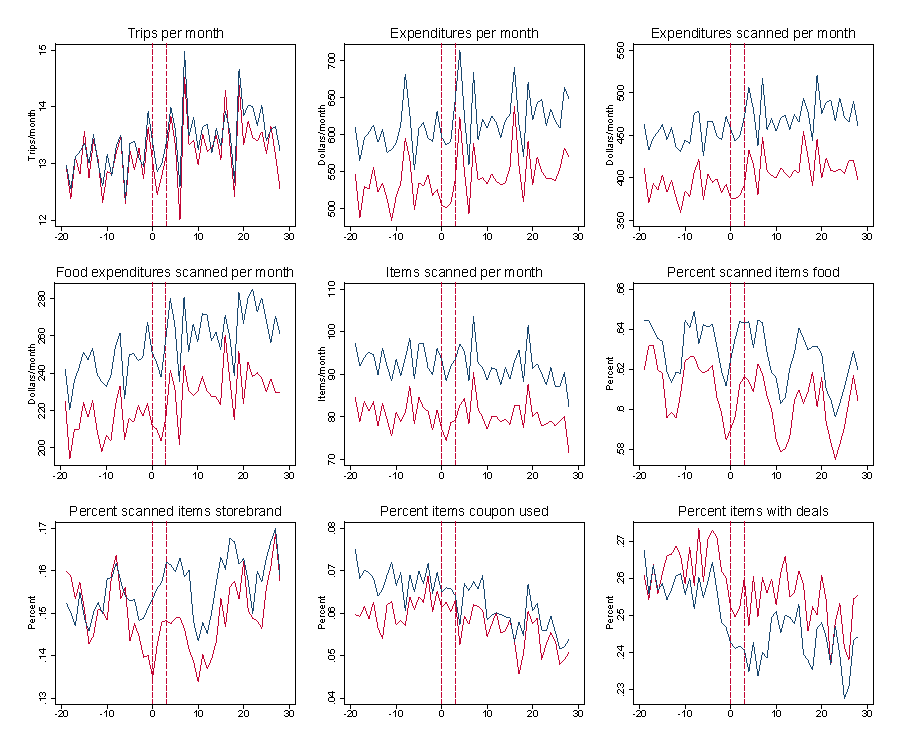
\includegraphics[width=1\textwidth, angle=0]{../figures/panelist_behav.pdf}
\footnotesize Each panel displays monthly sums or percentages for residents of Cook County, Illinois (red) and those in the same DMA outside of the county limits (blue). Vertical dashed lines represent the start and end of the tax in Cook County.
\end{center}
\end{figure}

% Cook Co: Panelist nutrition
\clearpage
\begin{figure}[t]
\begin{center}
\caption{Cook County DMA: nutrient composition over time}
\label{cook_panelist_nutr}
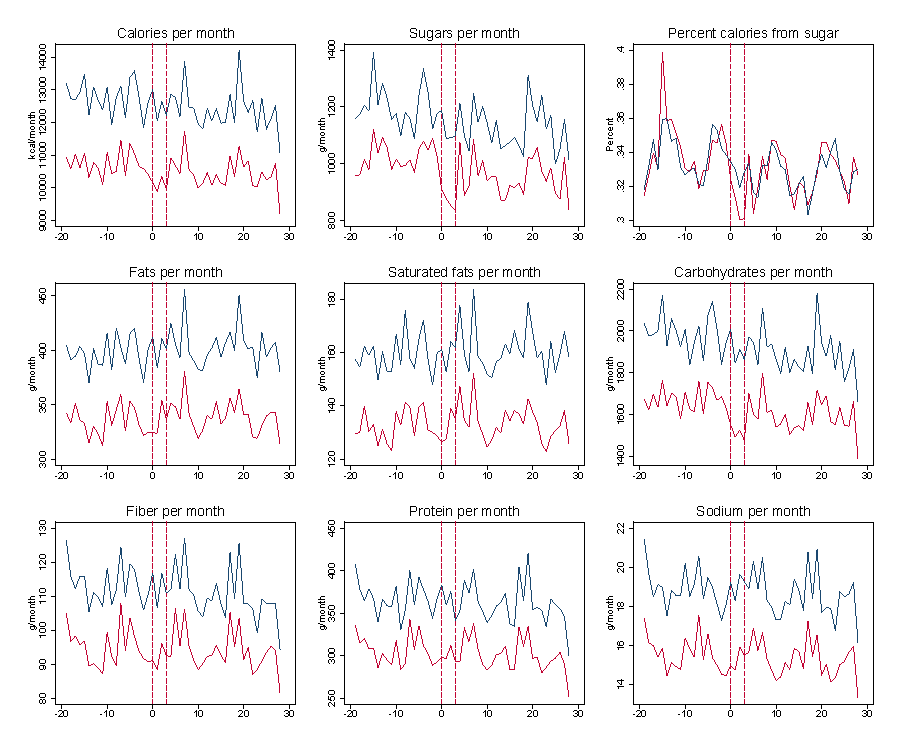
\includegraphics[width=1\textwidth, angle=0]{../figures/panelist_nutr.pdf}
\footnotesize Each panel displays monthly sums or percentages for residents of Cook County, Illinois (red) and those in the same DMA outside of the county limits (blue). Vertical dashed lines represent the start and end of the tax in Cook County.
\end{center}
\end{figure}

% Cook Co: Panelist beverages
\clearpage
\begin{figure}[t]
\begin{center}
\caption{Cook County DMA: beverage purchases over time}
\label{cook_panelist_nutr}
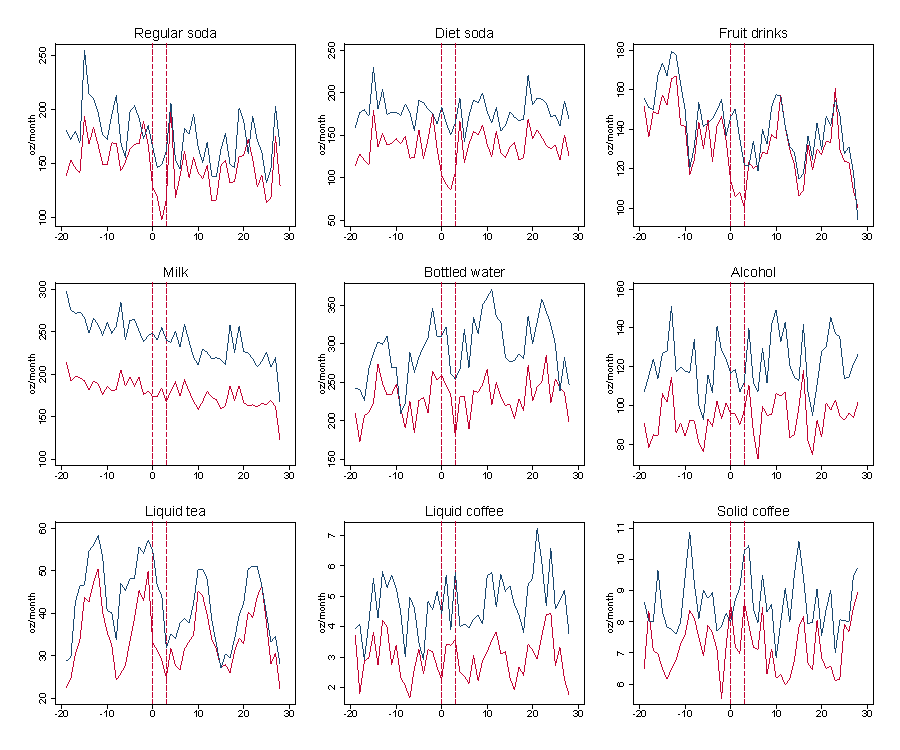
\includegraphics[width=1\textwidth, angle=0]{../figures/panelist_bev.pdf}
\footnotesize Each panel displays monthly sums of purchased beverages (in ounces) for residents of Cook County, Illinois (red) and those in the same DMA outside of the county limits (blue). Vertical dashed lines represent the start and end of the tax in Cook County.
\end{center}
\end{figure}

% Cook Co: nutrient coef plots
\clearpage
\begin{figure}[t]
\begin{center}
\caption{Effects of Cook County tax on nutrients purchased}
\label{cook_coef_combo}
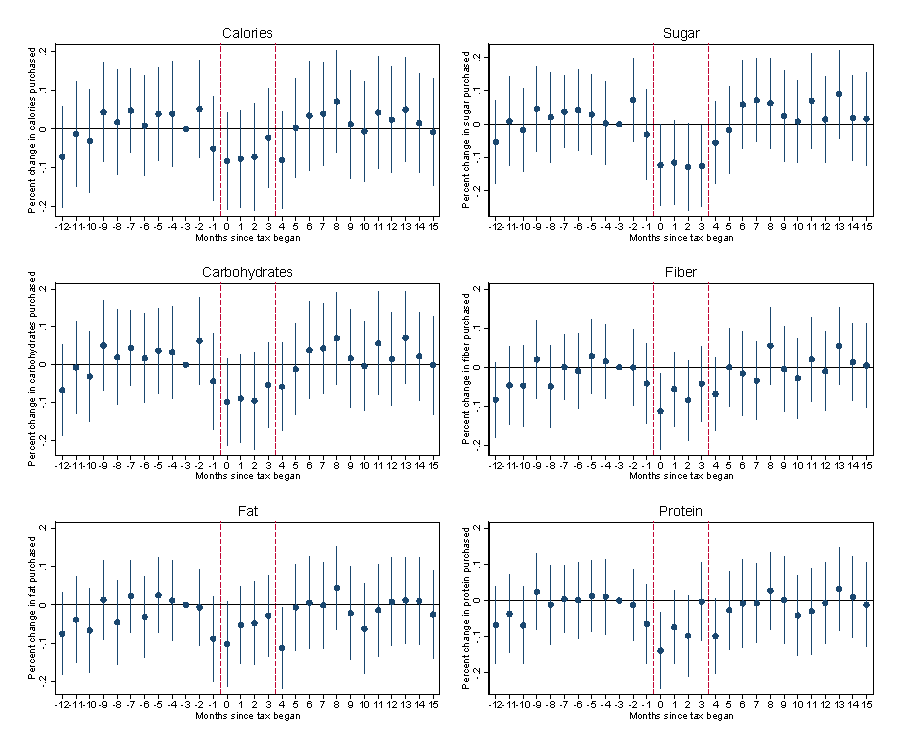
\includegraphics[width=1\textwidth, angle=0]{../figures/coefplot_cook_combo.pdf}
\footnotesize Each panel displays the monthly differences in log quantities purchased by residents of Cook County, Illinois and those in the same DMA outside of the county limits. The regressions used include household and month fixed-effects, and errors are clustered and the zip-code level. Vertical dashed lines represent the start and end of the tax in Cook County.
\end{center}
\end{figure}

\clearpage
\begin{figure}[t]\centering
  \caption{Cook County zip code layers} \label{cookzip}
	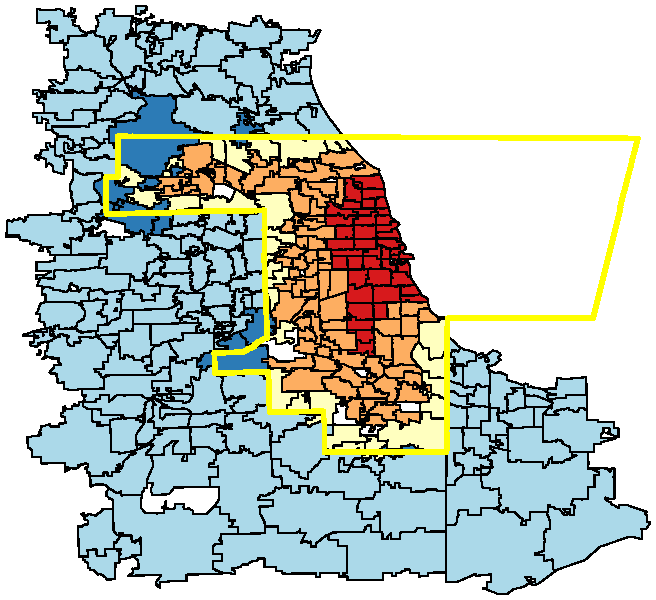
\includegraphics[width = \textwidth]{../figures/cookzips.pdf}
	\footnotesize Zip code layers used for examining heterogeneous treatment effects by distance from the nearest border. White regions in the map have no corresponding zip code information (lakes, forest, and other land without mailing addresses) and hence are excluded from the analysis. The darkest blue zip codes have houses both inside and outside Cook County's border. The lighter-yellow zips lie on the border entirely within Cook County. The remaining layers are constructed using linear distance to the nearest untaxed zip.
\end{figure}

% \clearpage
% \begin{figure}[t]\centering
% 	\includegraphics[width = \textwidth]{../figures/zip_tot_sugar.png}
% 	\caption{Impact of tax on sugar purchases as function of distance from the Cook County border. The omitted group is zips in the Chicago MSA entirely outside Cook County. \label{ziptotsugar}}
% \end{figure}

% \clearpage
% \begin{figure}[t]\centering
% 	\includegraphics[width = \textwidth]{../figures/zip_tot_sugar_soda.png}
% 	\caption{Impact of tax on purchases of sugar from soda as function of distance from the Cook County border. The omitted group is zips in the Chicago MSA entirely outside Cook County. \label{zipsugarsoda}}
% \end{figure}


% *****************************************************************
% Appendix
% *****************************************************************
\clearpage
\section*{Appendix}

\renewcommand{\thesubsection}{\Alph{subsection}}
\setcounter{table}{0}
\renewcommand{\thetable}{A\arabic{table}}
\setcounter{figure}{0}
\renewcommand{\thefigure}{A\arabic{figure}}

%%% TABLES

\clearpage
\begin{spacing}{1.0} \begin{table} \centering \caption{Effects of tax on sugar by pretreatment soda quintile, Boulder and Oakland} \label{sodatilesgoak} \begin{threeparttable} \begin{tabular}{m{0.23\linewidth}*{6}{>{\centering\arraybackslash}m{0.10\linewidth}}} \toprule
                    & \multicolumn{3}{c}{Months 1 - 4, sugar} & \multicolumn{3}{c}{Months 5 - 8, sugar}\\
\cmidrule(l{.75em}){2-4} \cmidrule(l{.75em}){5-7} 
Pre-tax soda quintile&\multicolumn{1}{c}{(1)}         &\multicolumn{1}{c}{(2)}         &\multicolumn{1}{c}{(3)}         &\multicolumn{1}{c}{(4)}         &\multicolumn{1}{c}{(5)}         &\multicolumn{1}{c}{(6)}         \\
\midrule
\customlinespace Quintile 1 &       0.004         &       0.009         &      -0.131         &       0.111         &      -0.029         &      -0.128         \\
                    &     (0.200)         &     (0.347)         &     (0.351)         &     (0.139)         &     (0.113)         &     (0.120)         \\
\customlinespace Quintile 2 &       0.148         &       0.021         &       0.074         &       0.514\sym{*}  &       0.508         &       0.496\sym{*}  \\
                    &     (0.203)         &     (0.215)         &     (0.307)         &     (0.205)         &     (0.277)         &     (0.244)         \\
\customlinespace Quintile 3 &      -0.220         &      -0.117         &      -0.129         &       0.095         &       0.088         &      -0.078         \\
                    &     (0.185)         &     (0.258)         &     (0.162)         &     (0.152)         &     (0.182)         &     (0.178)         \\
\customlinespace Quintile 4 &      -0.212         &      -0.304         &      -0.126         &      -0.175         &      -0.246         &      -0.735\sym{*}  \\
                    &     (0.199)         &     (0.281)         &     (0.332)         &     (0.298)         &     (0.310)         &     (0.333)         \\
\customlinespace Quintile 5 &       0.266         &       0.835\sym{**} &       0.749         &       0.175         &       0.643\sym{***}&       0.676\sym{***}\\
                    &     (0.194)         &     (0.287)         &     (0.385)         &     (0.142)         &     (0.174)         &     (0.175)         \\
\midrule
Treated Households           &          82         &          82         &          58         &          87         &          87         &          50         \\
Households          &        2059         &        2059         &        1306         &        2276         &        2276         &        1126         \\
Household-months    &       25883         &       25883         &       19590         &       32734         &       32734         &       21394         \\
Balanced Panel             &          No         &          No         &         Yes         &          No         &          No         &         Yes         \\
Sampling Weights             &          No         &         Yes         &         Yes         &          No         &         Yes         &         Yes         \\
\bottomrule \end{tabular} \Fignote{Coefficients represent the percent change in sugar purchased during the first four months (1 - 3) and second four months (4 - 6) after the Boulder and Oakland beverage taxes became active, separated by expenditure-weighted pretreatment regular soda volume purchase decile. Quintiles were calculated based on the treated households' average monthly volume of soda purchased during the previous year omitting the month prior to the tax. All of quintile 1 report zero regular soda purchases before the tax. \Regnote} \end{threeparttable} \end{table} \end{spacing}



%%% FIGURES

\begin{figure}[t]\centering
  \caption{Example price tag from Cook County grocery store} \label{pricetag}
	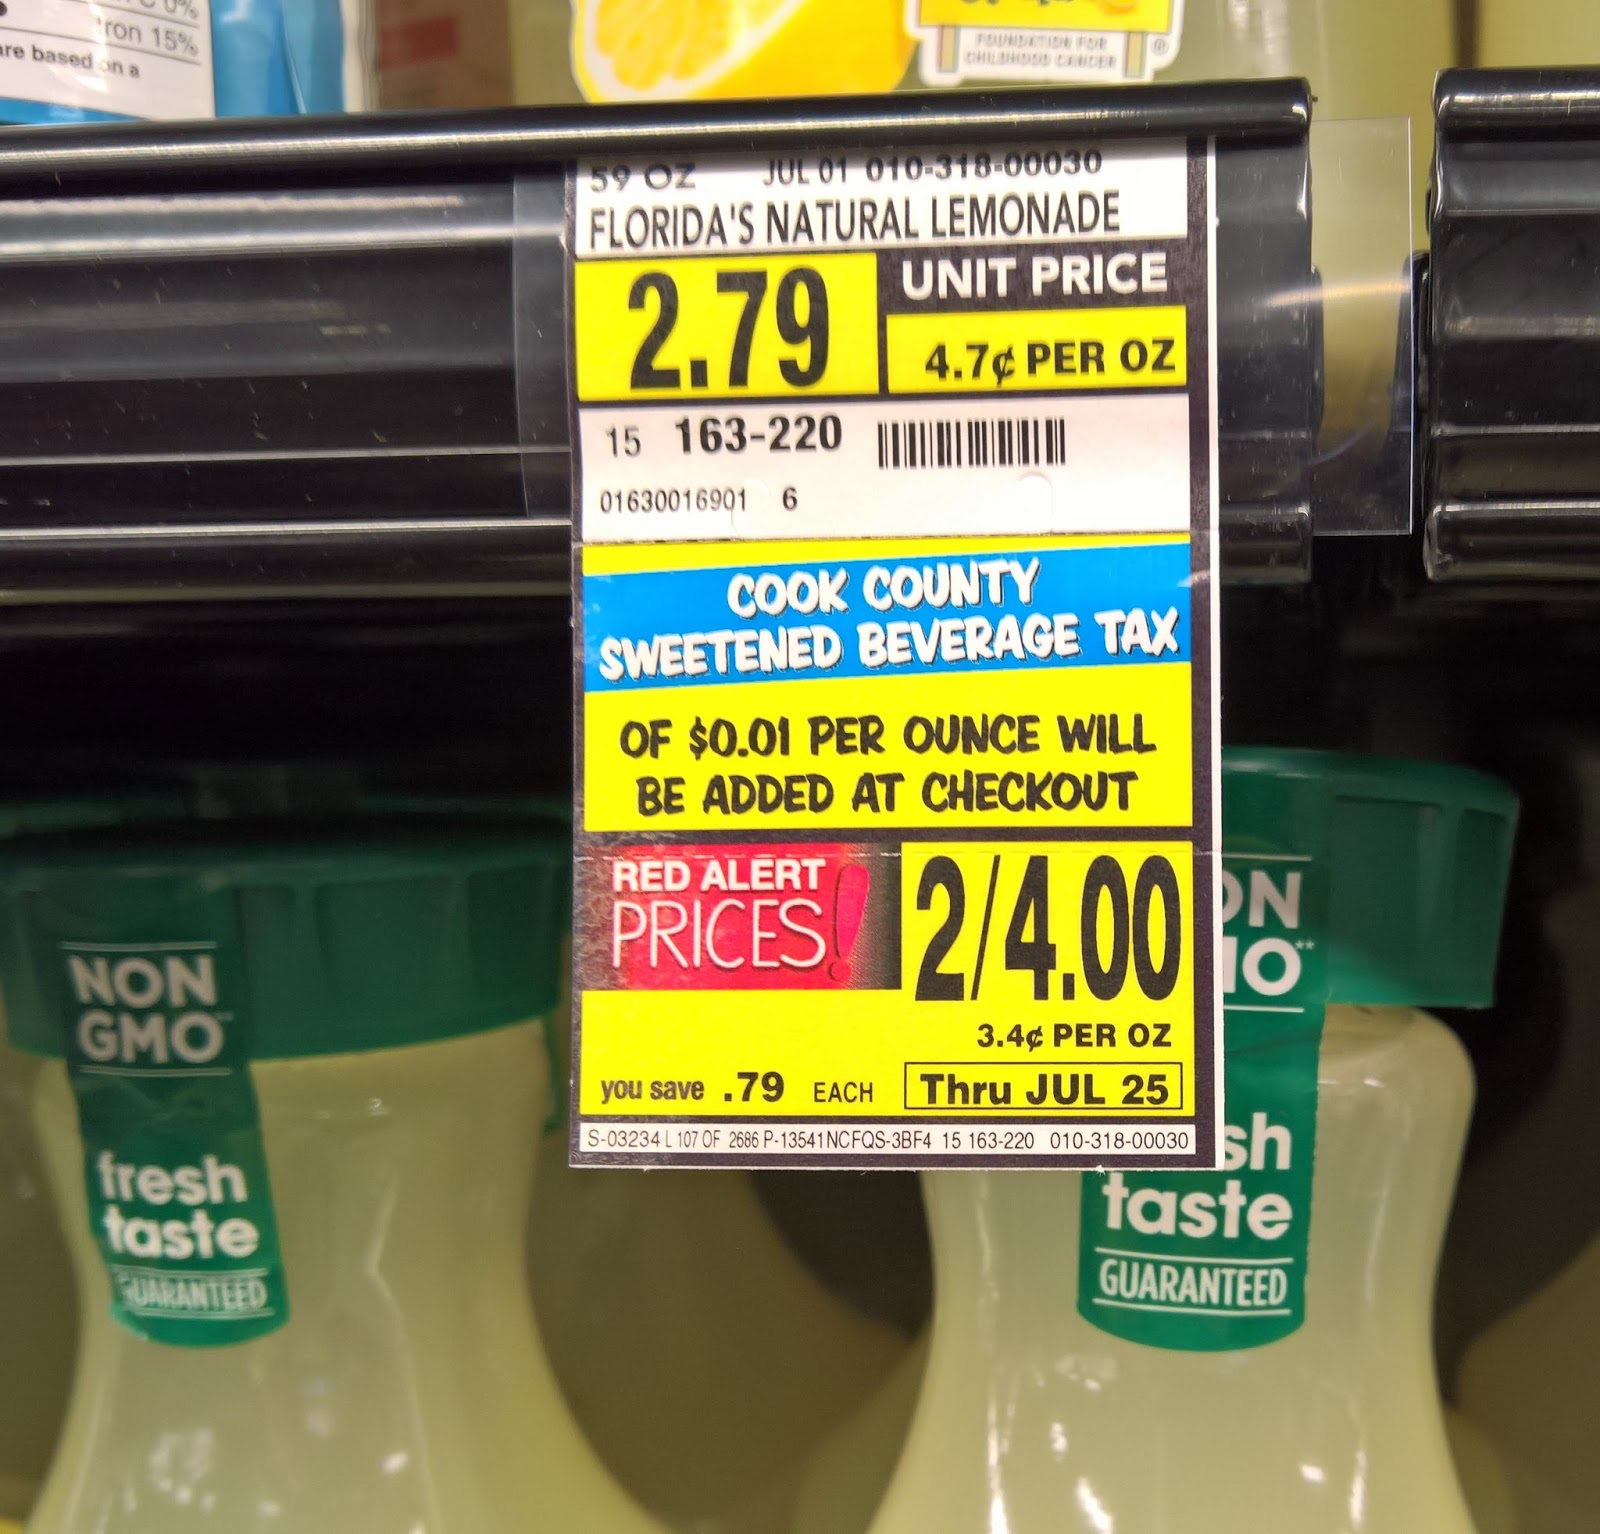
\includegraphics[width = \textwidth]{../figures/pricetag.jpg}
	\footnotesize This price tag includes a warning about the beverage tax in Cook County. Price tags like these may have increased salience of the tax whereas price tags in smaller, non-chain stores may not have.
\end{figure}

\clearpage
\begin{figure}[t]\centering
	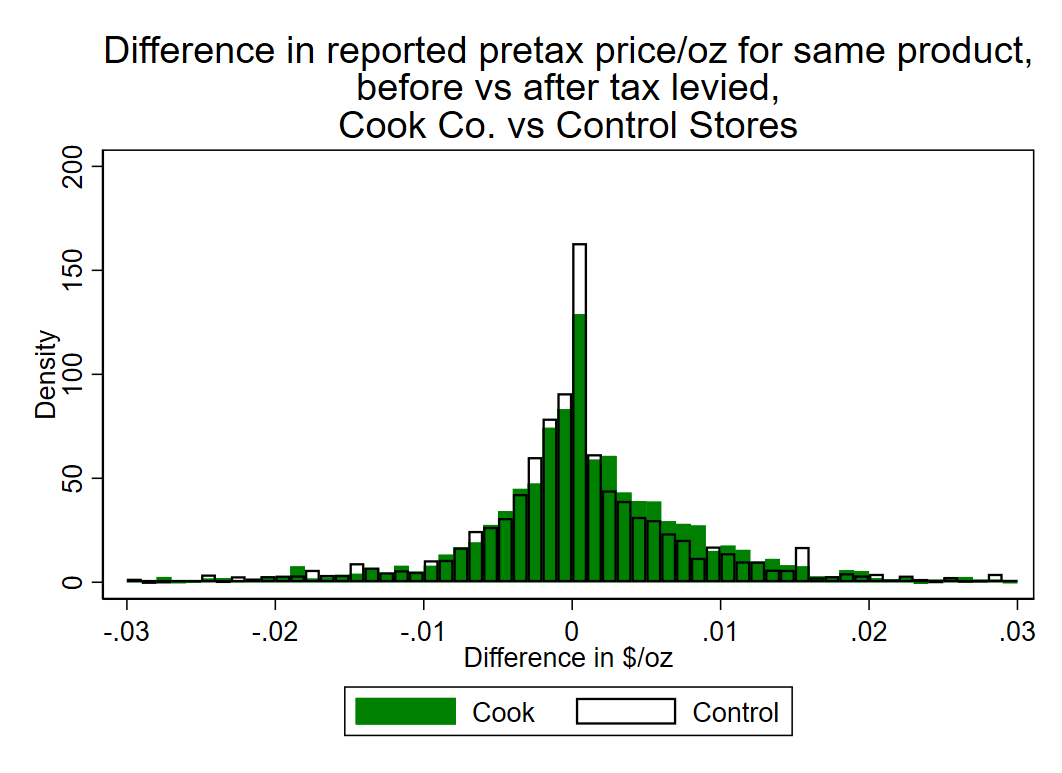
\includegraphics[width = \textwidth]{../figures/ppozdiff.png}\label{pricediff}
	\caption{Distribution of differences in price per ounce during pretax versus taxed periods for carbonated beverages}
\end{figure}

\clearpage
\begin{figure}[t]\centering
  \caption{Relative weekly search volume for ``soda tax"}
  \label{gtrends}
	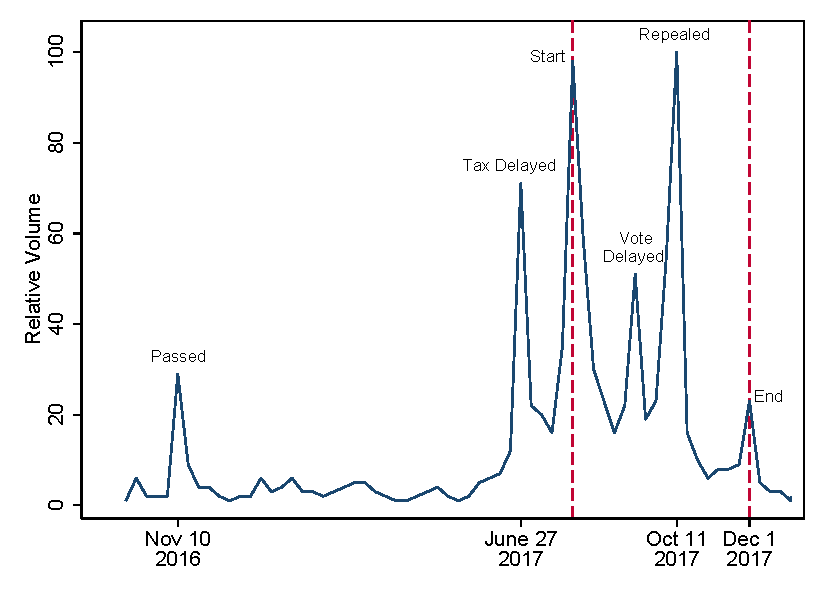
\includegraphics[width = \textwidth]{../figures/gtrends.pdf}
	\footnotesize This plot displays Google search volume in Illinois for the keywords ``soda tax". Each point is the volume in Illinois relative to the total search volume for that week in Illinois scaled so that the highest week's search volume is 100.
\end{figure}

\end{document}
